\documentclass[10pt, letterpaper]{article}
\usepackage{times} % changing font
\usepackage[greek,english]{babel}
\usepackage{alphabeta}
\usepackage{graphicx} % Required for inserting images
\usepackage{cite}
\usepackage{makecell}
\usepackage{todonotes}
\usepackage{cite}
\linespread{1.25} % 1.5 spacing
\pagenumbering{arabic}
\graphicspath{img}
\begin{document}
\renewcommand\refname{Αναφορές}
\renewcommand\contentsname{Περιεχόμενα}

    \begin{titlepage}

        \newcommand{\HRule}{\rule{\linewidth}{0.5mm}}
        
        \center
        
        \textsc{\LARGE Οικονομικό Πανεπιστήμιο Αθηνών}\\[1.5cm]
        \textsc{\large Ανάλυση Δεδομένων 2023 - Εργασία 4}\\[0.5cm]
        
        \HRule \\[0.4cm]
        {\huge Προεδρικες Εκλογές ΗΠΑ 2000: Μία Στατιστική Μελέτη και Ανάλυση }\\[0.4cm] 
        \HRule \\[1.5cm]
        
        \begin{minipage}{0.4\textwidth}
        \begin{flushleft} \large
        \emph{Ονοματεπώνυμο:}\\
        Ιωάννης Γκιώνης \textit{(p3190044)} \\
        \end{flushleft}
        \end{minipage}
        ~
        \begin{minipage}{0.4\textwidth}
        \begin{flushright} \large
        \emph{Διδάσκοντες:} \\
        Ι. Ντζούφρας, Ξ. Πεντελή \\
        \end{flushright}
        \end{minipage}\\[2cm]
        
        {\large 4 Ιουνίου 2023}\\[2cm]
        
        
\includegraphics[width=150px, keepaspectratio]{resources/logo_aueb.png}\\[1cm] 
        
        \vfill 
    
    \end{titlepage}

    \tableofcontents

    \newpage

    \section{Εισαγωγή – περιγραφή μελέτης και προβλήματος}

        \par Με την ραγδαία ανάπτυξη της επιστήμης της στατιστικής τις τελευταίες δεκαετίες, ένας τομέας της που έχει τραβήξει αρκετά το ενδιαφέρον του κόσμου είναι αυτός των δημοσκοπήσεων και των πολιτικών προβλέψεων. Με την ανάπτυξη καινούριων μεθόδων ανάλυσης δεδομένων, στατιστικών μοντέλων αλλά και αλγορίθμων μηχανικής μάθησης (Machine Learning) και βαθιάς μηχανικής μάθησης (Deep Learning), ο κλάδος αυτός έχει αποκτήσει πολλά καινούρια "εργαλεία" τα οποία βοηθούν τους data scientists να κάνουν την δουλειά τους πιο γρήγορα αλλά και πιο αποτελεσματικά. Η πρόβλεψη αποτελεσμάτων εκλογών είναι πολύ σημαντική, καθώς η κοινή γνώμη επηρεάζεται αρκετά από τις δημοσκοπήσεις και η τελική απόφαση ψήφου αρκετών ανθρώπων μπορεί να εξαρτάται σε κάποιο βαθμό από το τί αποτέλεσμα περιμένουν, άρα η σωστή συλλογή, επεξεργασία και απεικόνιση των δεδομένων είναι πολύ σημαντική.
        
        \par Η συγκεκριμένη μελέτη έχει ως αντικείμενο τις εκλογές των ΗΠΑ το 2000 και έχει ως σκοπό την έυρεση συσχέτισης ανάμεσα στα έτη διαμονής σε συγκεκριμένη πολιτεία και τις πολιτικές απόψεις/πρόθεση ψήφου των ερωτηθέντων. Επιπλέον, θα μελετηθεί το ενδεχόμενο κατασκευής γραμμικού μοντέλου πρόβλεψης του εισοδήματος ενός ερωτώμενου με δεδομένα ένα υποσύνολο των υπολοίπων μεταβλητών. Το σετ δεδομένων αποτελείται απο 1000 παρατηρήσεις 8 μεταβλητών και περιγράφεται στον πίνακα που βρίσκεται στην επόμενη σελίδα (σημείωση: η μεταβλητή ID παραλείπεται απο την υπόλοιπη μελέτη καθώς δεν μας προσφέρει καμία πληροφορία):
    
        \newpage

        \begin{center}
        \begin{table}[h!]
            \caption{Πίνακας Δεδομένων - Μεταβλητών}
            \label{summarytable}
            \begin{tabular}{||c|c|c|c|c||}
                \hline
                Όνομα & Τύπος & Σημασία & Τιμές - Εύρος Τιμών \\
                \hline
                ID & αριθμητική & Κωδικός ερωτώμενου & 1 - 1000 \\
                \hline
                Age & αριθμητική & Ηλικία & 18 - 90 \\
                \hline
                Years of residence & αριθμητική & \makecell{Πόσο καιρό μένει \\ κάποιος στην πολιτεία} & 0 - 72 \\
                \hline
                Income & αριθμητική & Ετήσιο Εισόδημα (σε δολάρια) & 2000 - 125000 \\
                \hline
                Gender & κατηγορική & Φύλο & Αρσενικό, Θηλυκό \\
                \hline
                Vote & κατηγορική & Ψήφος & \makecell{Al Gore \\ George W. Bush \\ Pat Buchanan \\ Ralph Nader \\ Other / Did Not Answer } \\
                \hline
                Political orientation & κατηγορική & Πολιτικές Πεποιθήσεις & \makecell{Extremely Liberal \\ Liberal, Slightly Liberal \\ Moderate \\ Slightly Conservative \\ Conservative \\ Extremely Conservative \\ Other / Did Not Answer }\\
                \hline
                Marital Status & κατηγορική & Οικογενειακή Κατάσταση & \makecell{Married, Widowed \\ Divorced, Separated \\ Never Married \\ Partnered \\ Other / Did Not Answer }\\
                \hline
            \end{tabular}
        \end{table}
        \end{center}
        
        \section{Περιγραφική Ανάλυση}

        \par Για την περιγραφική ανάλυση των μεταβλητών χρησιμοποιούμε το στατιστικό πακέτο R, το οποίο μας παρέχει εργαλεία για ανάλυση (Data Analysis) και απεικόνιση (Data Presentation) του σετ δεδομένων μας. Αρχικά, εισάγουμε τα δεδομένα μας μέσω του πακέτου Haven. Ύστερα, αφού κοιτάξουμε τη δομή του DataFrame, και εφόσον δεν θα χρειαστεί να αναλύσουμε κάτι σε κάποια συγκεκριμένη εγγραφή, διαγράφουμε την στήλη (Μεταβλητή) ID.

        \par Κοιτώντας τον πίνακα \ref{summarytable} εντοπίζουμε τις κατηγορικές μεταβλητές: Gender, Vote, Political Orientation, Marital Status και ορίζουμε τα κατάλληλα περιγραφικά μέτρα γι αυτές τα οποία επίσης απεικονίζονται στον παραπάνω πίνακα.\footnote{Σε κάποιες από τις παραπάνω μεταβλητές υπάρχουν μη-χρησιμοποιούμενες δεσμευμένες τιμές οι οποίες παραλείπονται από αυτή την ανάλυση καθώς δεν παρατηρούνται παραδείγματα που τις χρησιμοποιούν στο segment των δεδομένων που μας έχει δοθεί} Η κατηγορική μεταβλητή Gender είναι δίτιμη (0 = αρσενικό, 1 = θηλυκό), ενώ οι άλλες 3 έχουν πολλές τιμές, με την Political Orientation να είναι η μόνη η οποία μπορεί να θεωρηθεί διατάξιμη, με τις τιμές της(1-7) να βρίσκονται σε σειρά στο πολιτικό φάσμα από τον φιλελευθερισμό μέχρι τον συντηρητισμό.

        \par Συνεχίζοντας την ανάλυση αυτή τη φορα για ποσοτικές μεταβλητές, ελέγχουμε το εύρος τιμών κάθε μεταβλητής ξεχωριστά, κάνοντας ελέγχους Shapiro-Wilk\cite{shapiro} και Lillie\cite{lillie} για κανονικότητα. Παρακάτω ακολουθούν τα διαγράμματα πυκνότητας πιθανότητας για τις 3 ποσοτικές μεταβλητές (Age, Years of residence, Income) στα οποία περιέχονται τιμές των Shapiro tests καθώς και ένας πίνακας με τα περιγραφικά τους μέτρα.

        \begin{figure}[h!]
                \caption{Διαγράμματα Πυκνότητας Πιθανότητας}
                \label{densityplots}
                \centering
                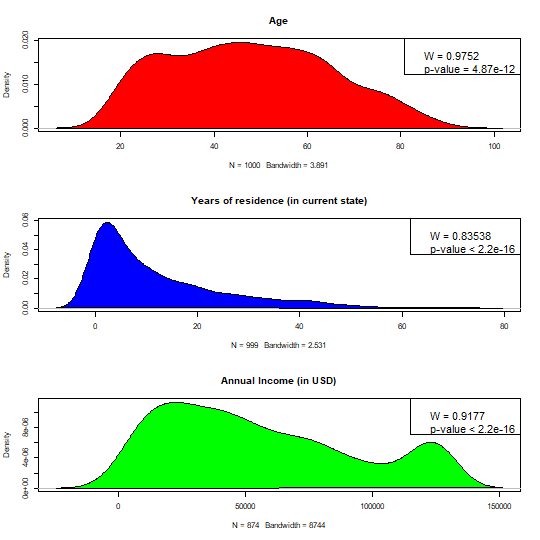
\includegraphics[width=300px, keepaspectratio]{resources/Density_Plots.png}
        \end{figure}
    
        \begin{table}[h!]
            \centering 
            \caption{Πίνακας Περιγραφικών Μέτρων Ποσοτικών Μεταβλητών} 
            \label{vartable} 
            \begin{tabular}{||c|c|c|c|c|c|c|c||}
                \hline
                Μεταβλητἠ & \makecell{Ελλιπείς \\ Τιμές} & Μέσος & \makecell{Τυπική \\ Απόκλιση} & \makecell{Ελάχιστη \\ Τιμή} & \makecell{Μέγιστη \\ Τιμή} & Ασσυμετρία & Κύρτωση \\
                \hline
                Age & 0 & 47.572 & 17.213 & 18 & 90 & 0.2 & -0.84 \\ 
                \hline
                Years of residence & 1 & 11.773 & 12.722 & 0 & 72 &  1.41 & 1.6 \\
                \hline
                Income & 126 & 55604 & 37649 & 2000 & 125000 & 0.54 & -0.87 \\ 
                \hline
            \end{tabular}
        \end{table} 

    \section{Σχέσεις Μεταβλητών ανα 2}

        \subsection{Γενικά}

            \par Αρχικά, μελετούμε τις σχέσεις ανάμεσα στις τρεις ποσοτικές μεταβλητές. Η μόνη που παρουσιάζει κάποια συσχέτιση είναι η $Age \sim Yearsofresidence$, καθώς στον έλεγχο Pearson παρουσιάζεται $pvalue \approx 0$ και $r=0.57$, το οποίο δείχνει μια θετική συσχέτιση, δηλαδή κατά κανόνα, όσο μεγαλύτερο γίνεται το Age, μεγαλώνει και το Years of residence. Στις άλλες 2 σχέσεις ($ Age \sim Income$ και $Years of residence \sim Income$) δεν παρατηρείται κάποια σημαντική συσχέτιση ανάμεσα στις μεταβλητές, ενώ τα pvalues των ελέγχων Pearson είναι 0.5 και 0.35 αντίστοιχα, άρα δεν μπορούμε να καταλήξουμε σε κάποιο συμπέρασμα.
            
            \par Ύστερα, κοιτώντας πίνακα συσχετίσεων του Pearson \ref{pearsonplot} βλέπουμε ότι υπάρχουν αρκετά μικρά p-values, άρα αρκετή συσχέτιση μεταβλητών στο σετ δεδομένων μας. Αγνοώντας τα ζέυγη μεταβλητών με υψηλά p-values και έχοντας υπ' όψην ότι οι μεταβλητές vote-political orientation και age-years of residency\footnote{οι υποθέσεις επιβεβαιώνονται απο ελέγχους $X^2$ και Pearson αντίστοιχα} σχετίζονται λογικά προσπαθούμε να βρούμε σχέσεις που θα βγάζουν νόημα να μελετηθούν. Οι σχέσεις:
            \begin{itemize}
                \item Χρόνια διαμονής σε πολιτεία και ψήφος ($Yearsofresidence \sim Vote$)
                \item Χρόνια διαμονής σε πολιτεία και πολιτικές πεποιθήσεις ($Yearsofresidence \sim PoliticalOrientation$)
            \end{itemize}
             θα μελετηθούν περαιτέρω στην ενότητα \ref{section::q2}. Τελικά, οι σχέσεις ανάμεσα σε ζεύγη μεταβλητών τις οποίες θα διερευνήσουμε είναι οι εξής:
    
            \begin{enumerate}
                \item Ετήσιο εισόδημα και φύλο ($Income \sim Gender$)
                \item Ηλικία και φύλο ($Age \sim Gender$)
                \item Ηλικία και οικογενειακή κατάσταση ($Age \sim Marital Status$)
                \item Ηλικία και ψήφος ($Age \sim Vote$)
                \item Ετήσιο Εισόδημα και οικογενειακή κατάσταση ($Income \sim Marital Status$)
                \item Πολιτικές πεποιθήσεις και οικογενειακή κατάσταση ($Political Orientation \sim Marital Status$)
                \item Ετήσιο εισόδημα και ψήφος ($Income \sim Vote$)
                \item Φύλο και ψήφος ($Gender \sim Vote$)
                \item Ψήφος και πολιτικές πεποιθήσεις ($Vote \sim Political Orientation$)
                \item Οικογενειακή κατάσταση και ψήφος ($Marital Status \sim Vote$)
                \item Ετήσιο εισόδημα και πολιτικές πεποιθήσεις ($Income \sim Poltical Orientation$)
            \end{enumerate}

            \par Τα διαγράμματα (barplots, boxplots) καθώς και τα αποτελέσματα των στατιστικών ελέγχων (Kruskal-Wallis test\cite{kruskalwallis} για ζέυγη ποσοτικών και κατηγορικών μεταβλητών και Chisquared \cite{pearsonchisq} + Fisher tests\cite{fisher} για ζέυγη κατηγορικών) βρίσκονται στο παράρτημα στην ενότητα \ref{section::appendix}. Από τις παραπάνω σχέσεις, αυτές που αποδείχθηκαν να έχουν κάποια στατιστικά σημαντική εξάρτηση μεταξύ τους είναι οι: 1,3,5,6,7,8,9,10,11 \footnote{$pvalue \leq 0.05$ σε ελέγχους kruskal ή chisq+fisher}
            
        \subsection{Συγκεκριμένες Σχέσεις Μεταβλητών}
        \label{section::q2}

            \par Σε αυτή την ενότητα θα αναλὐσουμε τις δὐο παρακάτω σχέσεις μεταξύ μεταβλητὠν:
            
            \begin{enumerate}
                \item Χρόνια διαμονής σε πολιτεία και ψήφος ($Yearsofresidence \sim Vote$)
                \item Χρόνια διαμονής σε πολιτεία και πολιτικές πεποιθήσεις ($Yearsofresidence \sim PoliticalOrientation$)
            \end{enumerate}

            \par Όπως παρατηρούμε και στον πίνακα \ref{summarytable}, και οι 2 σχέσεις πρόκειται για σχέσεις ποσοτικής και κατηγορικής μεταβλητής. Οι ελέγχοι που μπορούμε να εφαρμόσουμε είναι οι Kruskal test και ANOVA. Αρχικά κατασκευάζουμε τα αρχικά μοντέλα ANOVA και ύστερα τρέχουμε ελέγχους κανονικότητας και ομοσκεδαστικότητας\footnote{Τελικά δεν χρειάζεται έλεγχος ομοσκεδαστικότητας καθώς τα κατάλοιπα κανενός μοντέλου δεν ακολουθούν την κανονική κατανομη. Οι ελέγχοι γίνονται στον πηγαίο κώδικα και τα αποτελέσματά τους υπάρχουν σε comment}. Παρατηρούμε με ελέγχους Shapiro/Lillie ότι τα κατάλοιπα και των δύο μοντέλων δεν ακολουθούν την κανονική κατανομή, όπως άλλωστε φαίνεται στα διαγραμματα \ref{model1plot} και \ref{model2plot}. Επίσης από τα διαγράμματα παρατηρούμε και συμπαιρένουμε ότι ο διάμεσος είναι πιο κατάλληλο μέτρο περιγραφής έναντι του μέσου. Δίνουμε λοιπόν έμφαση στους ελέγχους Kruskal, τα αποτελέσματα των οποίων βρίσκονται παρακάτω.
            \begin{enumerate}
                \item $H=1.5788$, $df=4$, $pvalue=0.8126$, η $H_0$ δεν μπορεί να απορριφθεί.
                \item $H=18.082$, $df=6$, $pvalue=0.006$, η $H_0$ απορρίπτεται.
            \end{enumerate}

            \par Όπως φαίνεται από τα αποτελέσματα των ελέγχων Kruskal-Wallis, υπάρχει μια σημαντική εξάρτηση μεταξύ των δύο μεταβλητών της δεύτερης σχέσης, σε αντίθεση με αυτές της πρώτης. Δηλαδή, φαίνεται οι πολιτικές πεποιθήσεις ενός ανθρώπου να επηρεάζονται στατιστικά από το πόσο καιρό είναι κάτοικος της πολιτείας στην οποία μένει, ενώ το ίδιο δεν ισχύει για το την ψήφο του στις εκλογές του 2000.

            
    \section{Προβλεπτικά ή ερμηνευτικά μοντέλα}

        \par Για την κατασκευή ενός γραμμικού μοντέλου πρόβλεψης της πραγματικής τιμής της συνεχούς μεταβλητής Income χρειάζεται αρχικά να ελέγξουμε για τυχόν ακραίες τιμές (outliers). Μέσω του διαγράμματος \ref{incomeboxplot} αλλά και μέσω ελέγχων διαπιστώνουμε ότι δεν υπάρχουν τέτοιες τιμές στο σετ δεδομένων μας, οπότε είμαστε έτοιμοι να δούμε ποιές συσχετίσεις της μεταβλητής Income είναι αρκετά σημαντικές για να χρησιμοποιηθούν στο μοντέλο μας. Από την ανάλυση σχέσεων ανά 2 της προηγούμενης ενότητας βλέπουμε ότι ο συντελεστής συσχέτισης Pearson έχει χαμηλές απόλυτες τιμες (cor1= 0.022, cor2=-0.031) για τις συσχετίσεις $Income \sim Age$ και $Income \sim Years of residence$, ενώ τα μεγάλα p-values κάνουν αυτές τις μικρές συσχετίσεις ακόμα πιο ασήμαντες. Άρα, στα γραμμικά υποδείγματα που θα φτιαχθούν, δεν θα ληφθούν υπ' όψιν οι λοιπές συνεχείς αριθμητικές μεταβλητές. Στην επόμενη σελίδα βρίσκονται τα 4 boxplots για την μεταβλητή income και κάθε μια απο τις 4 κατηγορικές μεταβλητές. Γνωρίζουμε ήδη ότι η μεταβλητή Income είναι εξαρτημένη από όλες τις κατηγορικές μεταβλητές, δηλαδή τις: Gender, Vote, Marital Status και Political Orientation, κάτι το οποίο είναι εμφανές στα παρακάτω διαγράμματα.

        \newpage

        \begin{figure}[h!]
        \centering
            \begin{minipage}{.5\textwidth}
                \caption{Boxplot Ετήσιου Εισοδήματος και Ψήφου}
                \label{incomevoteplot}
                \centering
                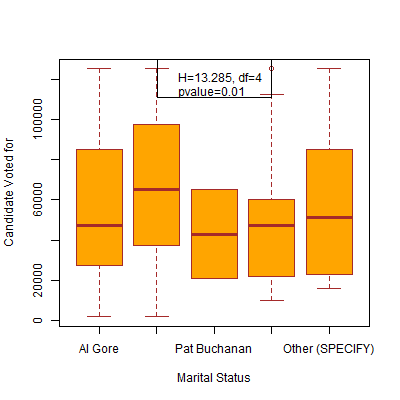
\includegraphics[width=0.9\linewidth]{resources/Income_Vote_Plot.png}
            \end{minipage}%
            \begin{minipage}{.5\textwidth}
                \caption{Boxplot Ετήσιου Εισοδήματος και Οικογενειακής Κατάστασης}
                \label{incomemaritalplot}
                \centering
                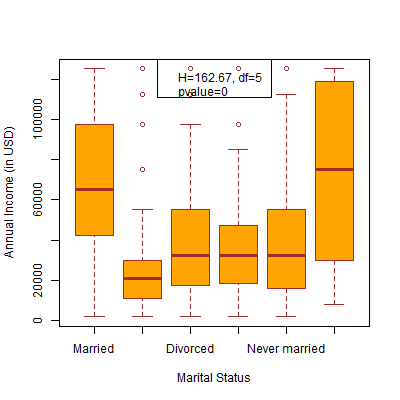
\includegraphics[width=0.9\linewidth]{resources/Income_MaritalStatus_Plot.png}
            \end{minipage}
            \label{boxplots1}
        \end{figure}
        \begin{figure}[h!]
        \centering
            \begin{minipage}{.5\textwidth}
                \caption{Boxplot Ετήσιου Εισοδήματος και Φύλου}
                \label{incomegenderplot}
                \centering
                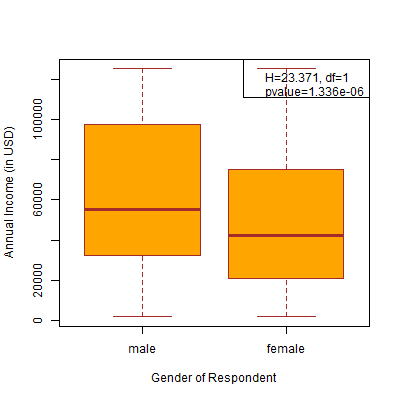
\includegraphics[width=0.9\linewidth, keepaspectratio]{resources/Income_Gender_Plot.png}
            \end{minipage}%
            \begin{minipage}{.5\textwidth}
                \caption{Boxplot Ετήσιου Εισοδήματος και Πολιτικού Προσανατολισμού}
                \label{incomepoliticalplot}
                \centering
                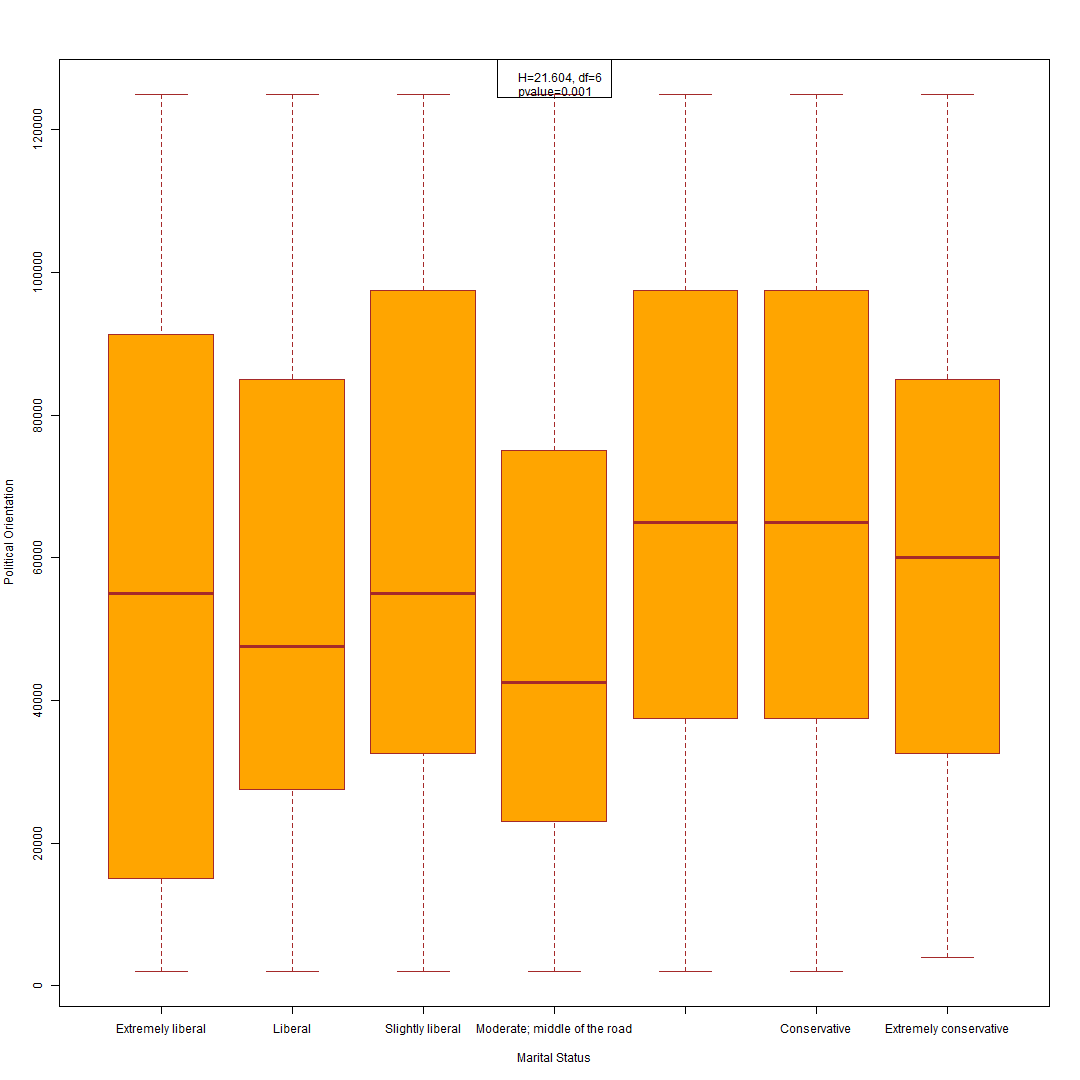
\includegraphics[width=0.9\linewidth]{resources/Income_PoliticalOrientation_Plot.png}
            \end{minipage}
            \label{boxplots2}
        \end{figure}
        
        \par Επιπλέον, παρατηρούμε στον έλεγχο $X^2$ που έγινε στις μεταβλητές Poltical Orientation και Vote ότι ο συντελεστής συσχέτισης $X^2$ ισούται με 279.7 και το pvalue ισούται με 0, το οποίο δείχνει μια πάρα πολύ σημαντική συσχέτιση των δύο μεταβλητών, κάτι που άλλωστε βγάζει νόημα λογικά. Επειδή οι δύο αυτές μεταβλητές εκφράζουν κάτι πάρα πολύ παρόμοιο και οι τιμές της μίας επηρεάζονται πάρα πολύ από τις τιμές της άλλης, θα χρησιμοποιήσουμε μόνο μία από τις 2 στα μοντέλα μας, έστω την Vote.

        \begin{table}[h!]
            \setlength\extrarowheight{-4pt}
            \caption{Πίνακας Πρώτου Μοντέλου Γραμμικής Παλλινδρόμισης} 
            \label{model1table} 
            \begin{tabular}{@{\extracolsep{5pt}}lc} 
                \\[-1ex]\hline 
                \hline \\[-1ex] 
                & \multicolumn{1}{c}{\textit{Dependent variable:}} \\ 
                \cline{2-2} 
                \\[-1ex] & Income \\ 
                \hline
                \hline \\[-1ex] 
                Gender: female & $-$7,916.522$^{***}$ \\ 
                & (2,920.591) \\ 
                & \\ 
                Vote: George W. Bush & 4,728.246 \\ 
                & (2,936.674) \\ 
                & \\ 
                Vote: Pat Buchanan & 653.727 \\ 
                & (24,382.570) \\ 
                & \\ 
                Vote: Ralph Nader & $-$6,980.956 \\ 
                & (9,164.055) \\ 
                & \\ 
                Vote: Other (SPECIFY) & $-$1,432.393 \\ 
                & (14,132.430) \\ 
                & \\ 
                Marital\_Status: Widowed & $-$33,862.190$^{***}$ \\ 
                & (5,609.388) \\ 
                & \\ 
                Marital\_Status: Divorced & $-$25,634.470$^{***}$ \\ 
                & (4,222.485) \\ 
                & \\ 
                Marital\_Status: Separated & $-$25,586.400$^{***}$ \\ 
                & (8,516.669) \\ 
                & \\ 
                Marital\_Status: Never married & $-$22,148.090$^{***}$ \\ 
                & (4,006.045) \\ 
                & \\ 
                Marital\_Status: Partnered, not married \{VOL\} & 26,435.220$^{**}$ \\ 
                & (12,296.670) \\ 
                & \\ 
                \hline
                \hline \\[-1ex] 
                Observations & 593 \\ 
                R$^{2}$ & 0.170 \\ 
                Adjusted R$^{2}$ & 0.156 \\ 
                Residual Std. Error & 34,147.320 (df = 582) \\ 
                F Statistic & 11.922$^{***}$ (df = 10; 582) \\ 
                & \\ 
                \hline 
                \hline \\[-1ex] 
                \textit{Note:}  & \multicolumn{1}{r}{$^{*}$p$<$0.1; $^{**}$p$<$0.05; $^{***}$p$<$0.01} \\ 
                \hline
            \end{tabular} 
        \end{table}

        \newpage
        \par Κατασκευάζουμε το γραμμικό μοντέλο παλλινδρόμησης με τις 3 μεταβλητές\footnote{η συνάρτηση lm() του προγραμματιστικού περιβάλλοντος R κατασκευάζει από μόνη της ψευδομεταβλητές για τις κατηγορικές μεταβλητές που του δίνουμε, όπως άλλοστε φαίνεται και στον πίνακα \ref{model1table}} ($Income \sim Gender + Marital Status + Vote $. Όπως και θα παρατηρήσουμε στον παραπάνω πίνακα, όλες οι τιμές της μεταβλητής Vote παίρνουν πολύ μεγάλα pvalues($<0.1$), άρα δοκιμάζουμε να κατασκευάσουμε ένα αντίστοιχο μοντέλο χωρίς την μεταβλητή Vote. Ο αντίστοιχος πίνακας γι΄ αυτό το μοντέλο καθώς και τα αντίστοιχα QQPlots των καταλοίπων των δύο μοντέλων βρίσκονται στο παράρτημα. Για την σύγκριση των δύο μοντέλων χρησιμοποιούμε έλεγχο ANOVA, τα αποτελέσματα του οποίου μας δείχνουν ότι τα δύο μοντέλα είναι πολύ παρόμοια, άρα θα κρατήσουμε ως βέλτιστο αυτό με τις λιγότερες μεταβλητές, άρα το δεύτερο. Ελέγχουμε τις προϋποθέσεις παλλινδρόμησης κάνοντας ελέγχους κανονικότητας (Shapiro/Lillie) στα κατάλοιπα αλλά και ελέγχους ομοσκεδαστηκότητας Levene\cite{levene}, μέσω των οποίων καταλήγουμε στο συμπέρασμα ότι τα κατάλοιπα δεν ειναι κανονικά και υπάρχει ομοσκεδαστηκότητα αλλά όχι σε μεγάλο βαθμό. Για να επιβεβαιώσουμε ότι το μοντέλο που κατασκευάσαμε είναι το βέλτιστο, τρέχουμε μια step-wise function\footnote{Χρησιμοποιούμε modified dataframe με τις 3 μεταβλητές που έχουν μείνει. Εάν χρησιμοποιήσουμε το αρχικό dataframe το αποτέλεσμα θα είναι παρόμοιο αλλά η περικοπή εγγραφών λόγω null values σε irrelevant στήλες οδηγεί σε χαμηλότερο $R_{adj}^2$, άρα δεν είναι η καλύτερη επιλογή} η οποία μας επιστρέφει το βέλτιστο μοντέλο, το οποίο φαίνεται πως είναι ακριβώς το ίδιο με το δέυτερο μοντέλο που κατασκευάσαμε. Είναι χρήσιμο να σημειωθεί ότι ακόμα και το βέλτιστο προβλεπτικό μοντέλο δεν έχει μεγάλη ακρίβεια, καθώς το στατιστικό $R_{adj}^2$ ισούται με 0.156, ενώ το $R^2$ ισούται με 0.165.

        \par Συμπερασματικά, το βέλτιστο μοντέλο είναι αυτό που χρησιμοποιεί μόνο τις κατηγορικές μεταβλητές Gender και Marital Status. Εάν θεωρήσουμε εξίσωση γραμμικής παλινδρόμησης $Income_{pred} = b0 + b1GenderFemale + b2MaritalWidowed + b3MaritalDivorced + b4Separated + b5NeverMarried + b6Partnered$ με default values τα Gender = Male και Marital Status = Married, τότε οι συντελεστές ισούνται με: $b0=76984$, $b1 = -8128$, $b2 = -34629$, $b3 = -26518$, $b4 = 26468$, $b5 = -23403$, $b6 = 25128$, άρα πρακτικά αυτό που καταλαβαίνουμε από το μοντέλο είναι ότι ο μέσος παντρεμένος άντρας βγάζει 76984 δολλάρια το χρόνο, ποσό που μειώνεται εάν μιλάμε για γυναίκα, για χωρισμένο/-η κλπ με μόνη περίπτωση αύξησης να απαντάται στην περίπτωση που η οικογενειακή κατάσταση ισούται με Partnered/Not Married, περίπτωση που απαντάται πολύ λιγες φορές στο dataset μας, κάτι που επιβεβαιώνεται από το pvalue που ισούται με 0.04, τιμή η οποία βρίσκεται ακριβώς πάνω στα όρια του στατιστικά σημαντικού.
    
    \section{Συμπεράσματα}

    \par Η στατιστική μελέτη αυτή είχε ως σκοπό την πλήρη ανάλυση των μεταβλητών του σετ δεδομένων καθώς και των μεταξύ τους συσχετίσεων αλλά και την κατασκευή ενός γραμμικού μοντέλου με σκοπό την πρόβλεψη του ετησίου εισοδήματος ενός αμερικάνου πολίτη με βάση τα λοιπά στοιχεία που υπάρχουν στο σετ δεδομένων. Ενώ το μοντέλο έχει αρκετά χαμηλές τιμές $R^2$ και $R^2_{adj}$ (0.165 και 0.156 αντίστοιχα), κάτι που δείχνει ότι η προσαρμογή του μοντέλου δεν είναι και η καλύτερη, καταφέρνει αρκετά καλά να περιγράψει τις συσχετίσεις που υπάρχουν στο σετ δεδομένων.

    \par Από το αρχικό μοντέλο, φαίνεται πόσο δυνατές είναι οι συσχετίσεις με τις 2 κατηγορικές μεταβλητές που τελικά καταλήγουμε να χρησιμοποιούμε, καθώς τα pvalues τους στον πίνακα \ref{model1table} είναι πολύ κοντά στο 0, σε αντίθεση με τις υπόλοιπες μεταβλητές. Επίσης, από το τελικό μοντέλο φαίνεται το πόσο σημαντικό ρόλο παίζει η οικογένεια στην δυτική της μορφή στο τελικό εισόδημα ενός ανθρώπου, καθώς παρατηρείται ότι οι γυναίκες, παρόλο που θεσμικά πληρώνονται ακριβώς το ίδιο με τους άντρες, καταλήγουν να έχουν αρκετά χαμηλότερο ετήσιο εισόδημα, γεγονός που αποδίδεται συνήθως στις αυξημένες ευθύνες και στον μειωμένο χρόνο λόγω της ιδιότητας των γυναικών ως μητέρες αλλά και την μεγαλύτερη συμβολή τους στα οικιακά. Επιπλέον, παρατηρείται διαφορά στο εισόδημα ανάμεσα σε ανθρώπους διαφορετικών οικογενειακών καταστάσεων, αλλά το μέγεθος του δείγματος, το πλήθος των διαφορετικών τιμών(6) αλλά και το γεγονός ότι το μεγαλύτερο κομμάτι του δείγματος παίρνει μια συγκεκριμένη τιμή (παντρεμένος/-η) δεν μας αφήνει να βγάλουμε κάποιο πραγματικό συμπέρασμα.

    \newpage
    \section{Παράρτημα}
    \label{section::appendix}
        \begin{center}
            \begin{figure}[h]
                \caption{Πίνακας Συσχετίσεων του Pearson}
                \label{pearsonplot}
                \centering
                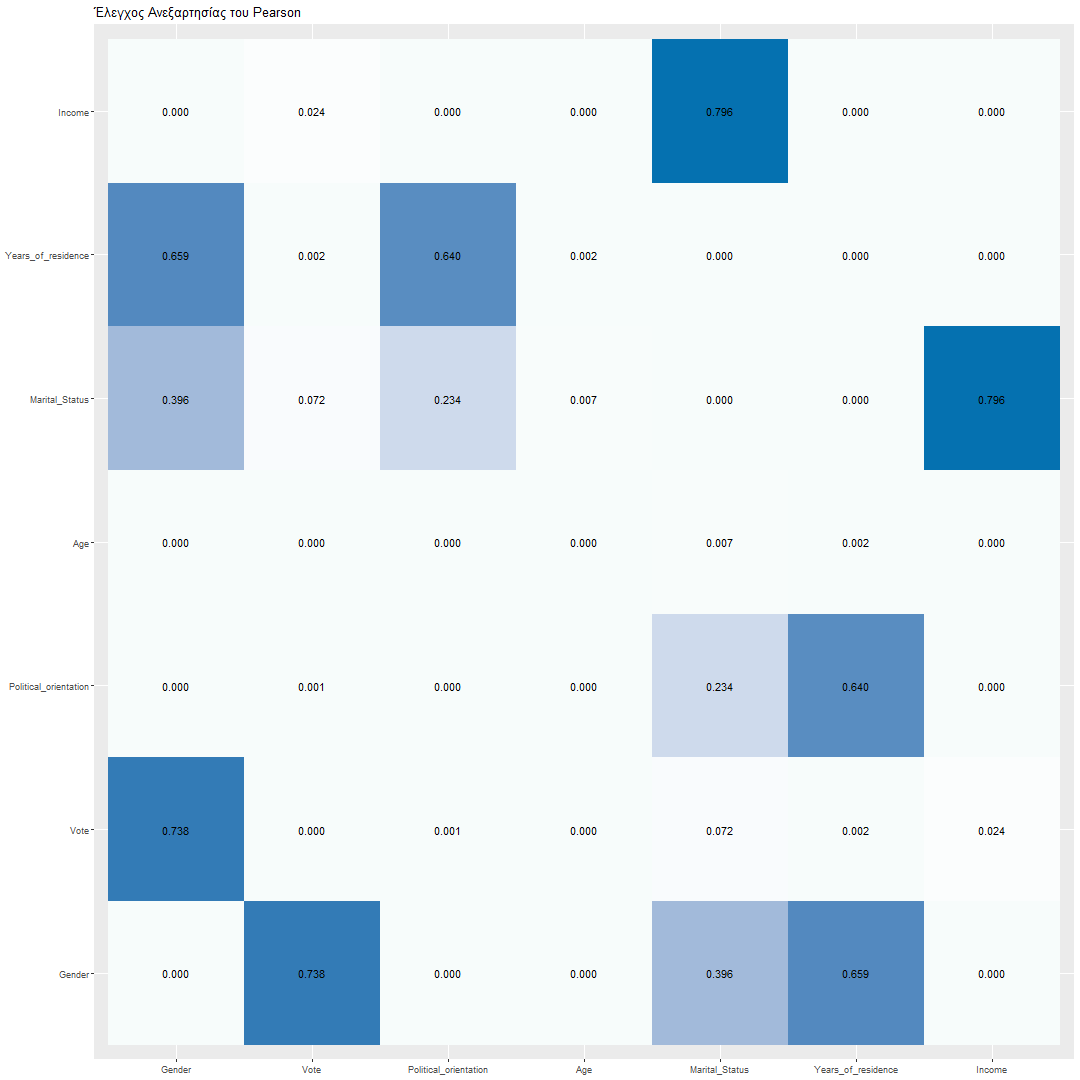
\includegraphics[width=300px, keepaspectratio]{resources/Pearson_Plot.png}
            \end{figure}
            \newpage
            \begin{figure}[h]
                \caption{Διάγραμμα (Boxplot) Ετήσιου Εισοδήματος}
                \label{incomeboxplot}
                \centering
                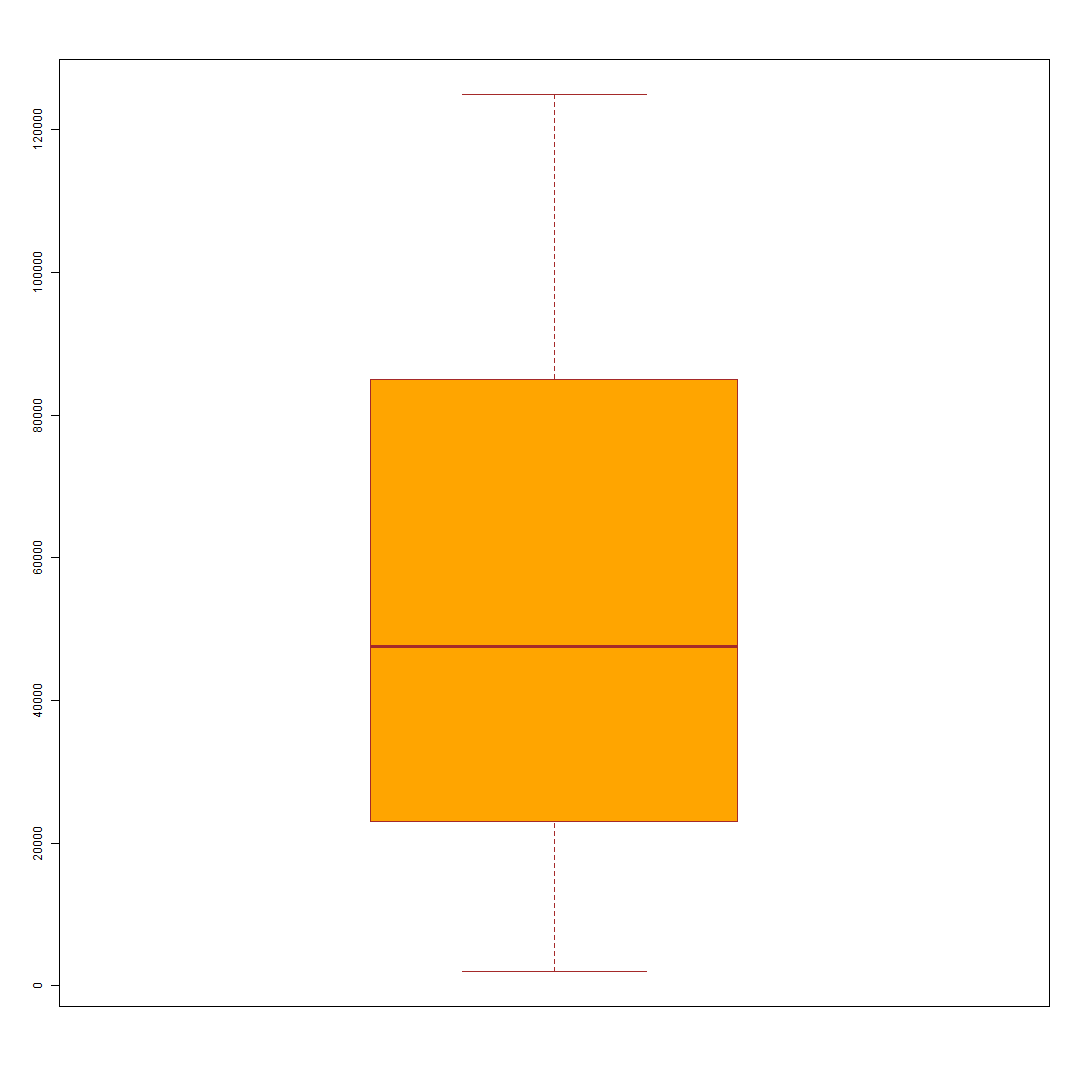
\includegraphics[width=300px, keepaspectratio]{resources/Income_Boxplot.png}
            \end{figure}
            \newpage
            \begin{figure}[h]
                \caption{Διάγραμμα Διασποράς Ηλικίας και Χρόνων διαμονής σε πολιτεία}
                \label{ageyearplot}
                \centering
                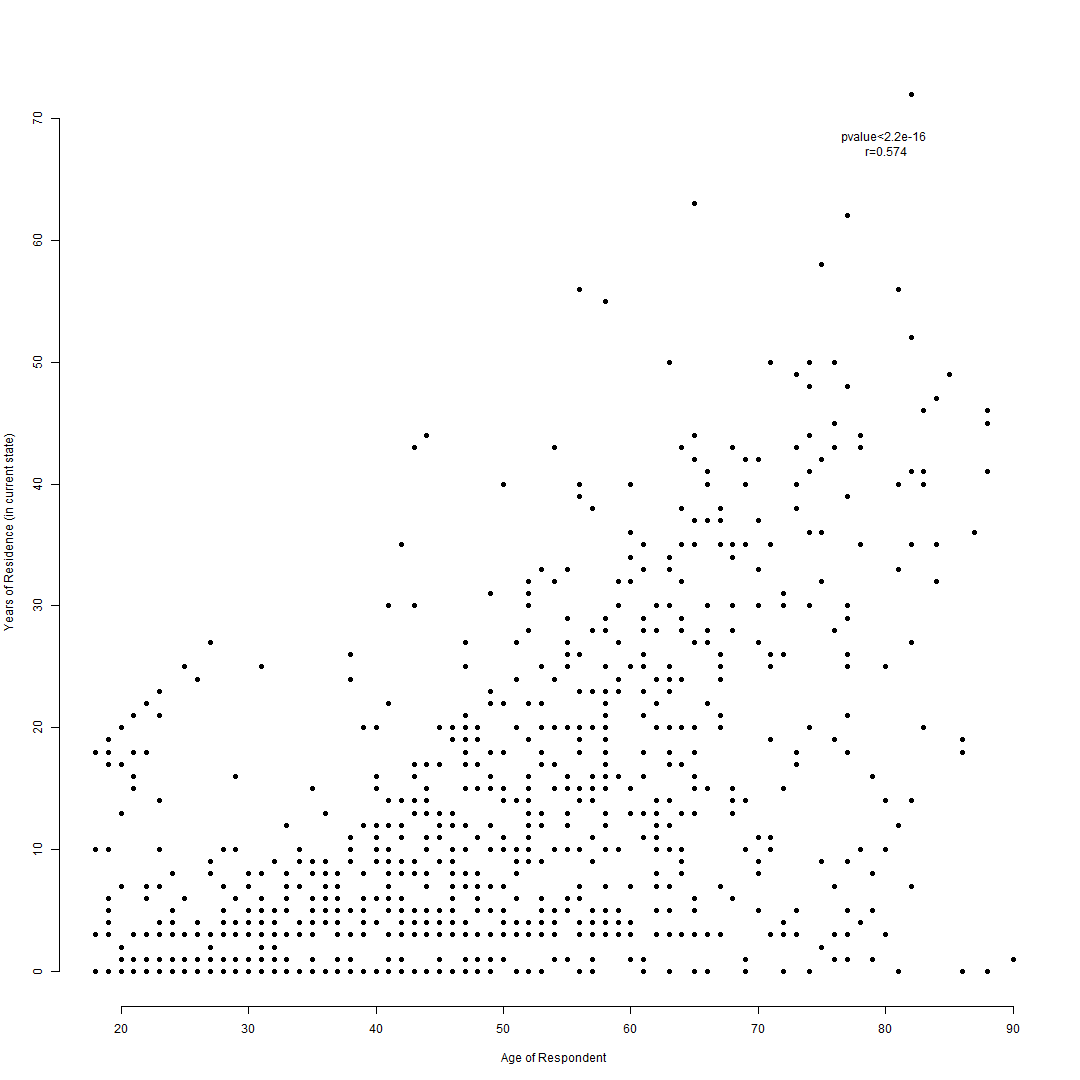
\includegraphics[width=300px, keepaspectratio]{resources/Age_YearsOfResidency_Plot.png}
            \end{figure}
            \newpage
            \begin{figure}[h]
                \caption{Διάγραμμα Διασποράς Ηλικίας και Ετήσιου Εισοδήματος}
                \label{ageincomenplot}
                \centering
                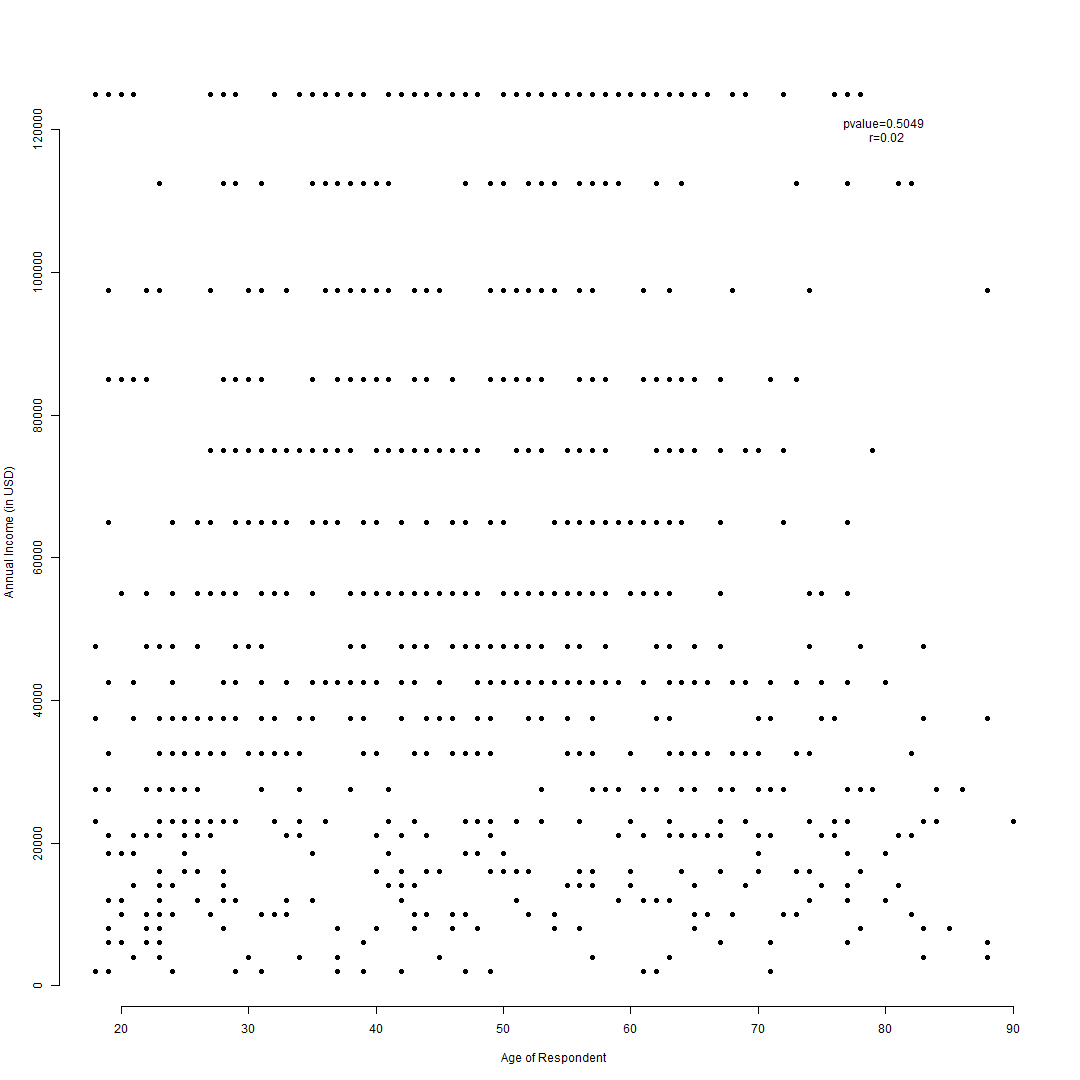
\includegraphics[width=300px, keepaspectratio]{resources/Age_Income_Plot.png}
            \end{figure}
            \newpage
            \begin{figure}[h]
                \caption{Διάγραμμα Διασποράς Χρόνων διαμονής σε πολιτεία και Ετήσιου Εισοδήματος}
                \label{yearsincomeplot}
                \centering
                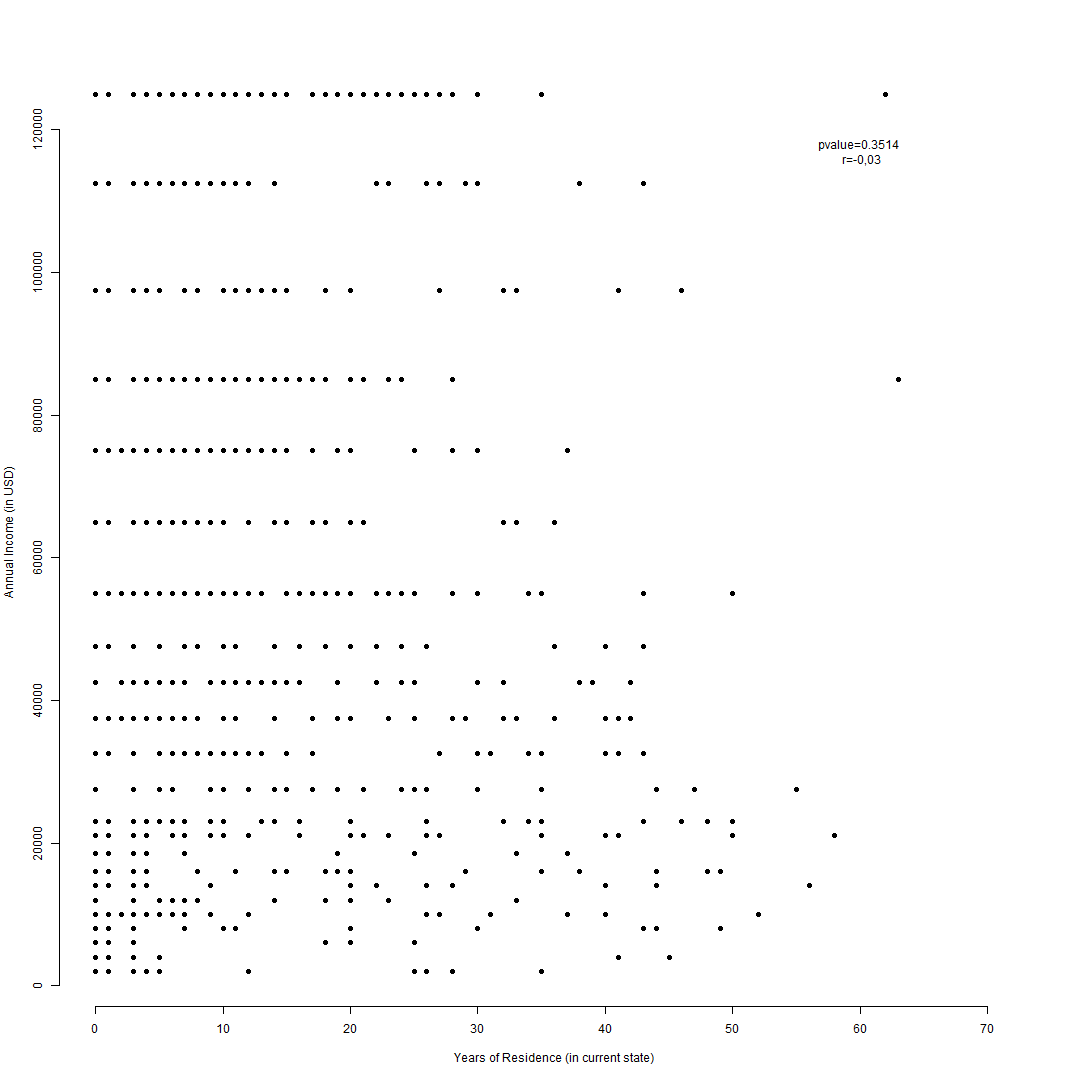
\includegraphics[width=300px, keepaspectratio]{resources/YearsOfResidence_Income_Plot.png}
            \end{figure}
            \newpage
            \begin{figure}[h]
                \caption{Boxplot Ηλικίας και Φύλου}
                \label{agegenderplot}
                \centering
                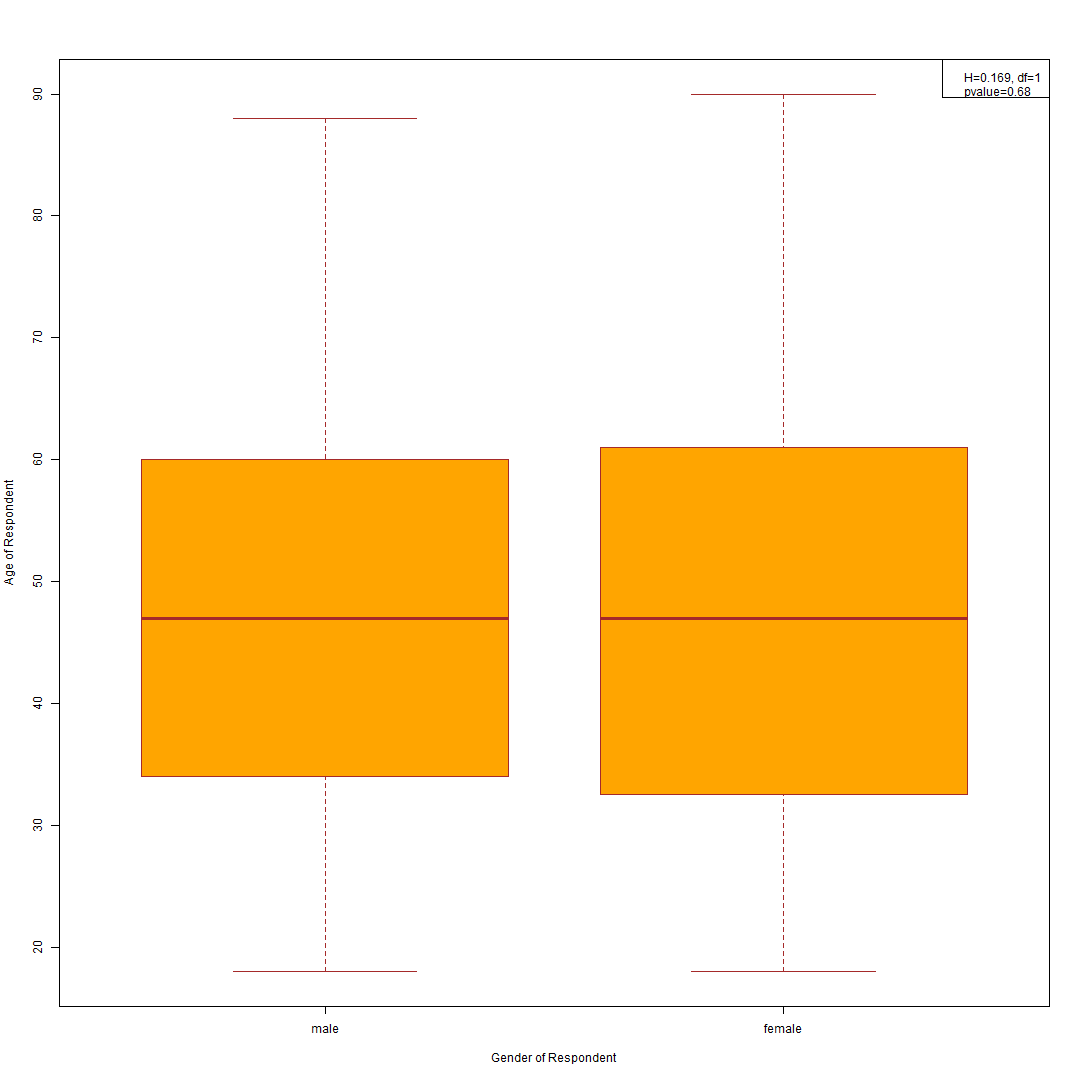
\includegraphics[width=300px, keepaspectratio]{resources/Age_Gender_Plot.png}
            \end{figure}
            \newpage
            \begin{figure}[h]
                \caption{Boxplot Ηλικίας και Οικογενειακής Κατάστασης}
                \label{agemaritalplot}
                \centering
                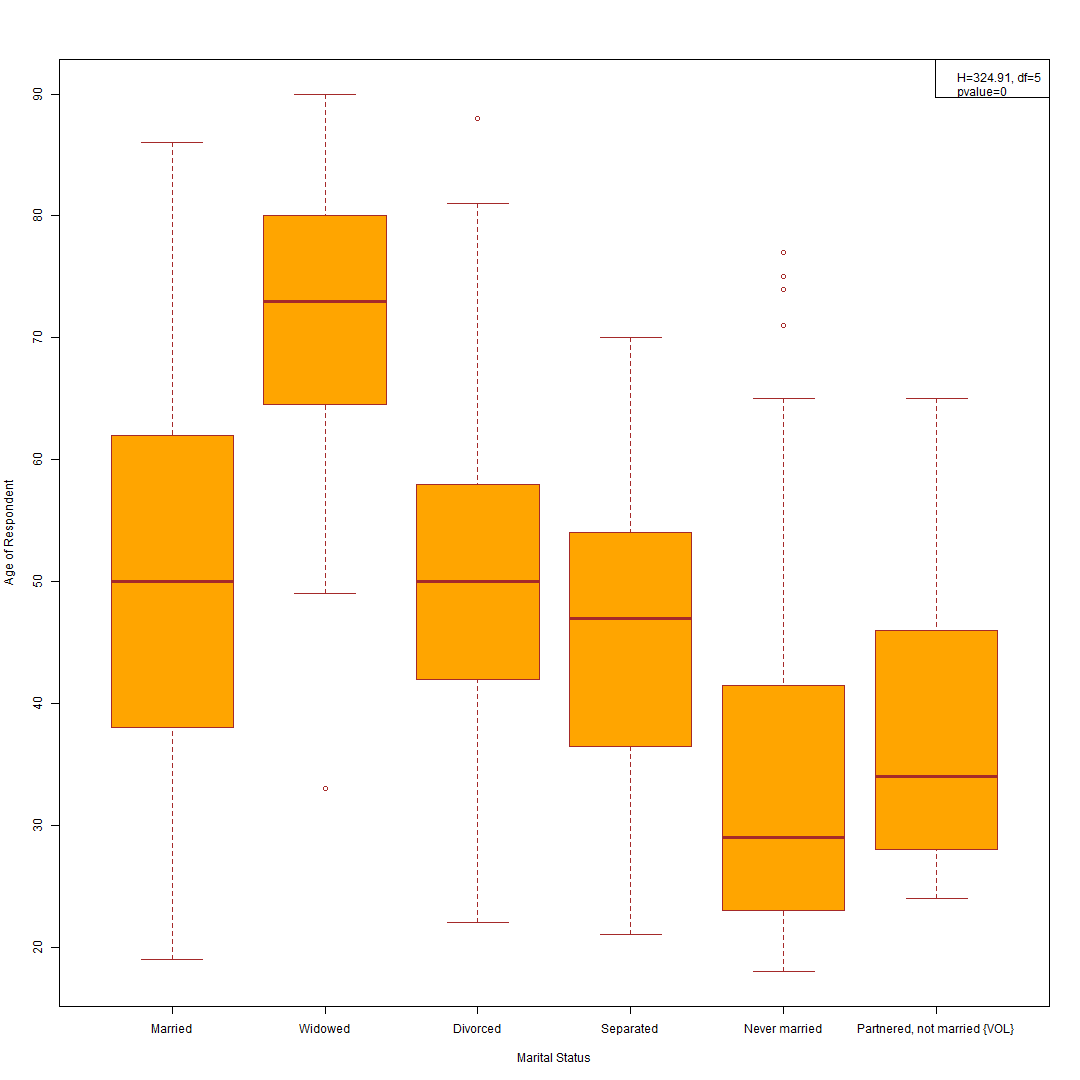
\includegraphics[width=300px, keepaspectratio]{resources/Age_MaritalStatus_Plot.png}
            \end{figure}
            \newpage
            \begin{figure}[h]
                \caption{Boxplot Ηλικίας και Ψήφου}
                \label{agevoteplot}
                \centering
                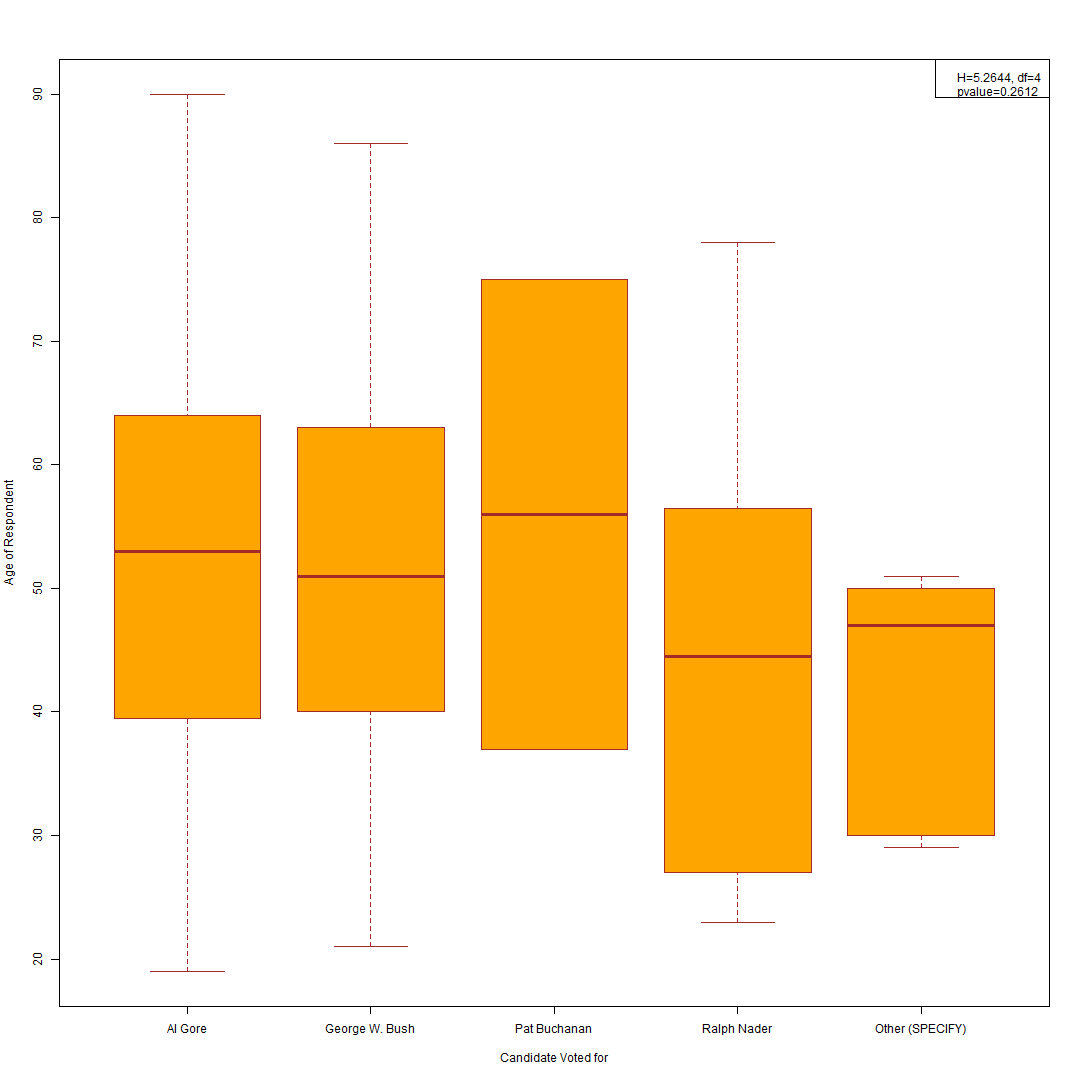
\includegraphics[width=300px, keepaspectratio]{resources/Age_Vote_Plot.png}
            \end{figure}
            \newpage
            \begin{figure}[h]
                \caption{Barplot Φύλου και Ψήφου}
                \label{gendervoteplot}
                \centering
                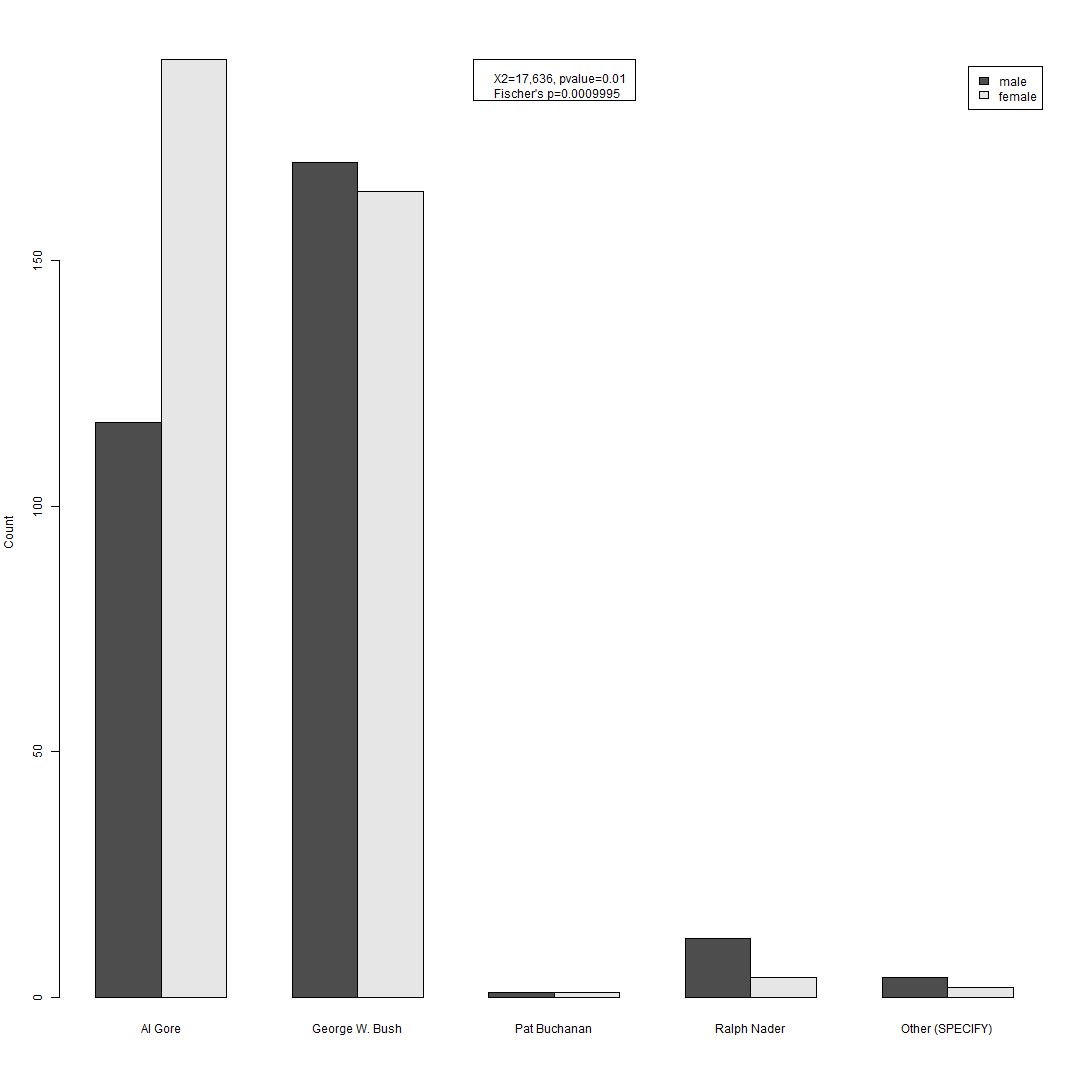
\includegraphics[width=300px, keepaspectratio]{resources/Gender_Vote_Plot.png}
            \end{figure}
            \newpage
            \begin{figure}[h]
                \caption{Barplot Πολιτικών Πεποιθήσεων και Οικογενειακής Κατάστασης}
                \label{politicalmaritalplot}
                \centering
                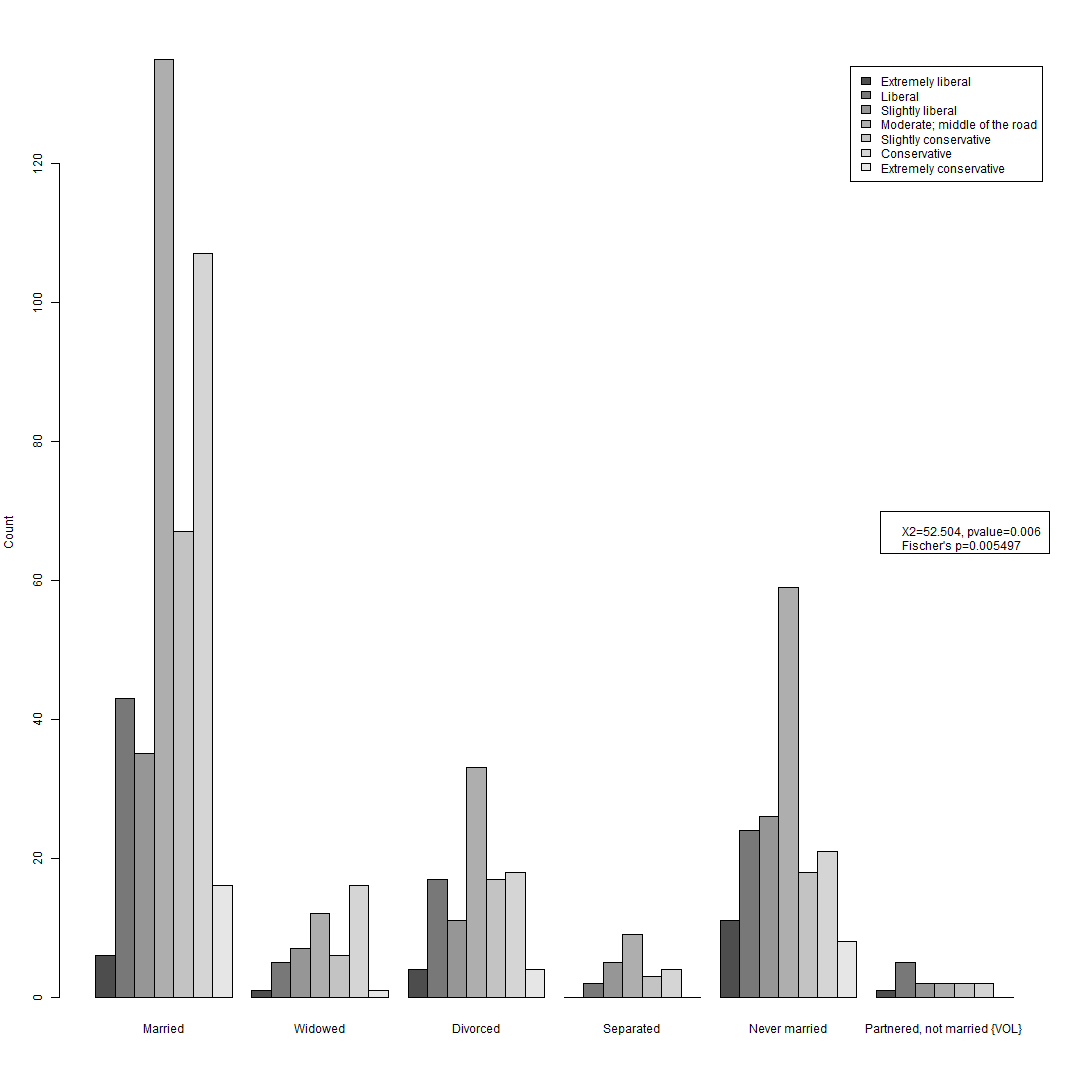
\includegraphics[width=300px, keepaspectratio]{resources/PoliticalOrientation_MaritalStatus_Plot.png}
            \end{figure}
            \newpage
            \begin{figure}[h]
                \caption{Barplot Ψήφου και Πολιτικών Πεποιθήσεων}
                \label{votepoliticalplot}
                \centering
                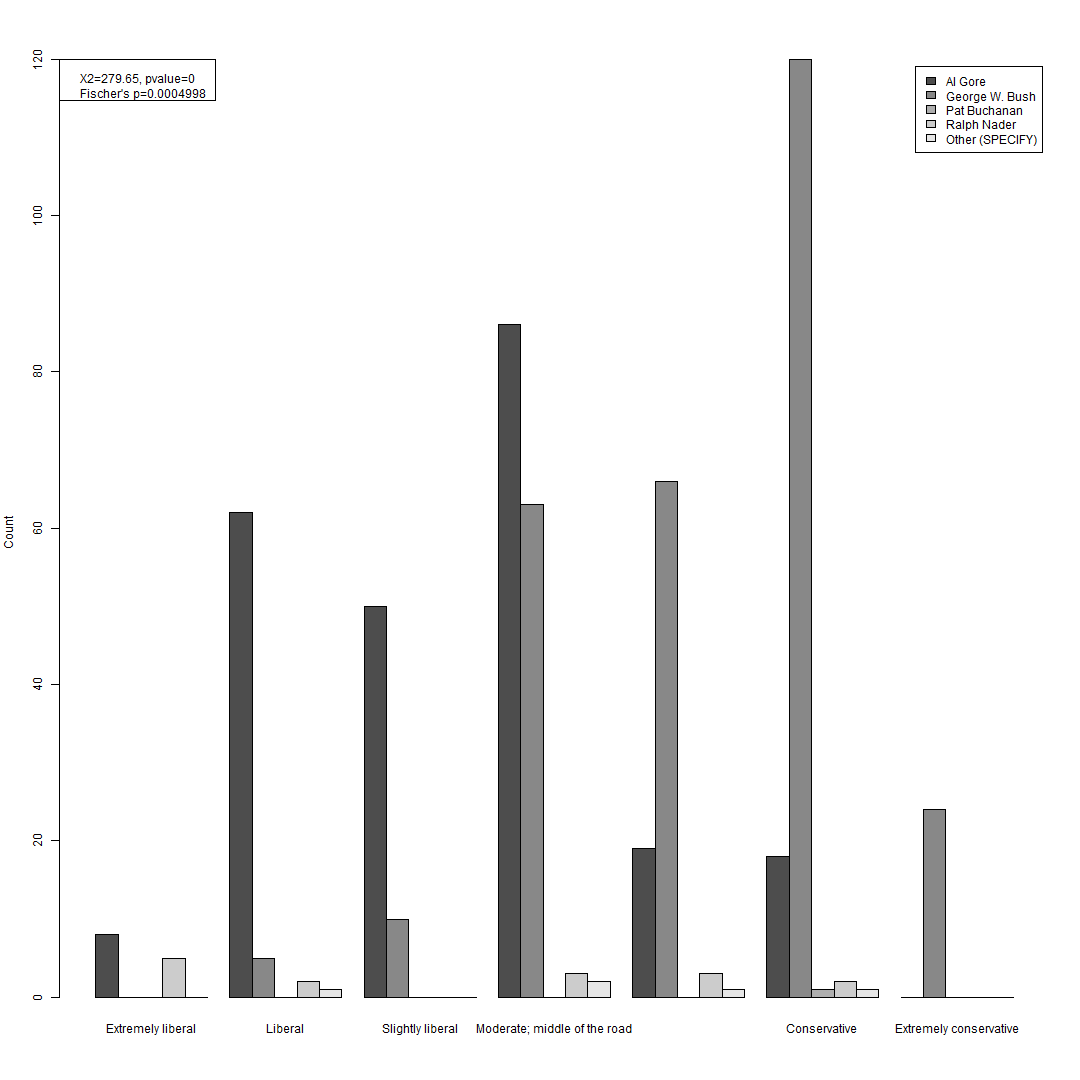
\includegraphics[width=300px, keepaspectratio]{resources/Vote_PoliticalOrientation_Plot.png}
            \end{figure}
            \newpage
            \begin{figure}[h]
                \caption{Barplot Οικογενειακής Κατάστασης και Ψήφου}
                \label{maritalvoteplot}
                \centering
                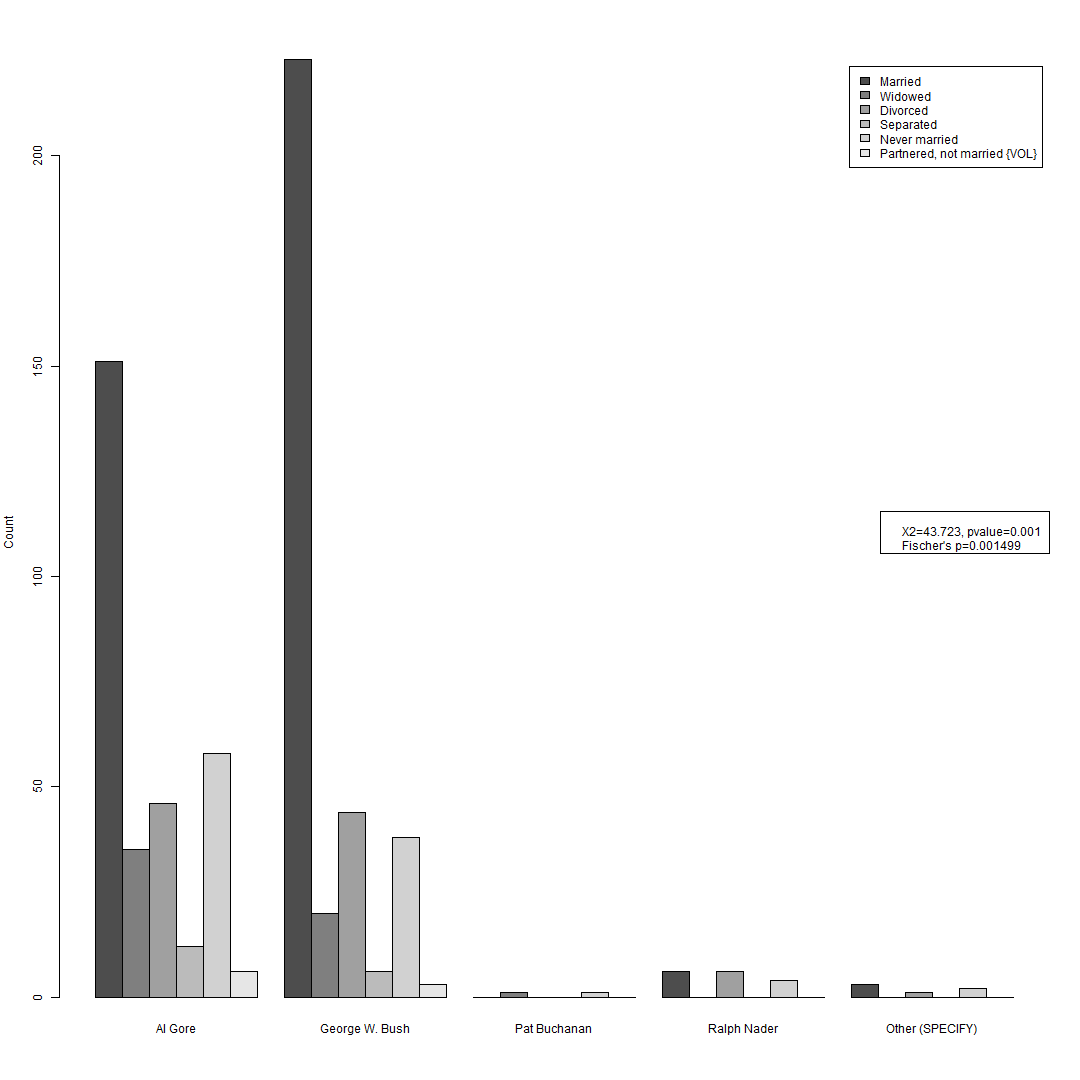
\includegraphics[width=300px, keepaspectratio]{resources/MaritalStatus_Vote_Plot.png}
            \end{figure}
            \newpage
            \begin{figure}[h]
                \caption{Barplot Ετών Διαμονής σε πολιτεία και Ψήφου}
                \label{yearsvoteplot}
                \centering
                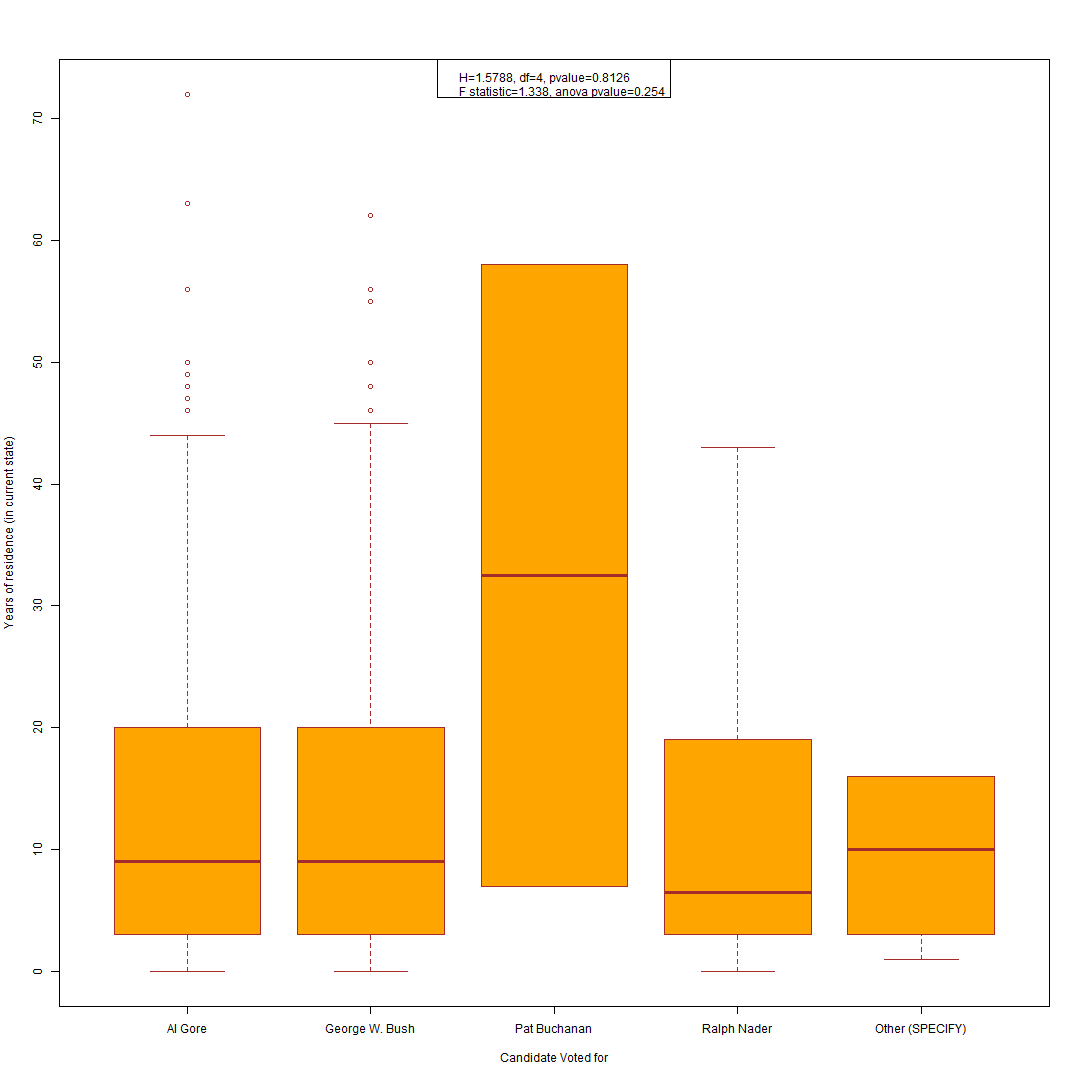
\includegraphics[width=300px, keepaspectratio]{resources/YearsOfResidence_Vote_Plot.png}
            \end{figure}
            \newpage
            \begin{figure}[h]
                \caption{Barplot Ετών Διαμονής σε πολιτεία και Πολιτικών Πεποιθήσεων}
                \label{yearspoliticalplot}
                \centering
                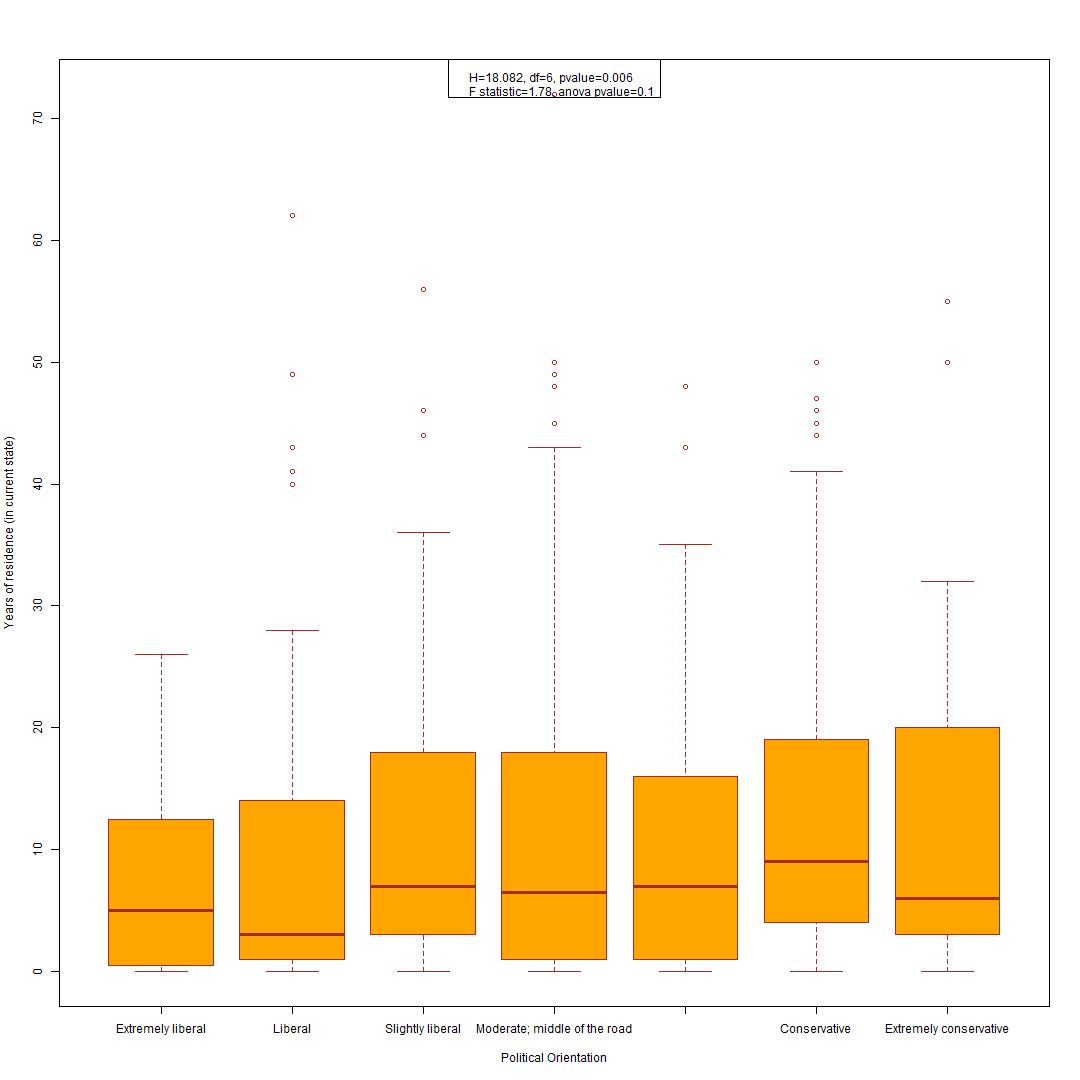
\includegraphics[width=300px, keepaspectratio]{resources/YearsOfResidence_PoliticalOrientation_Plot.png}
            \end{figure}
            \newpage
            \begin{figure}[h]
                \caption{QQPlot Μοντέλου ANOVA1 ($Yearsofresidence \sim Vote$)}
                \label{anova1plot}
                \centering
                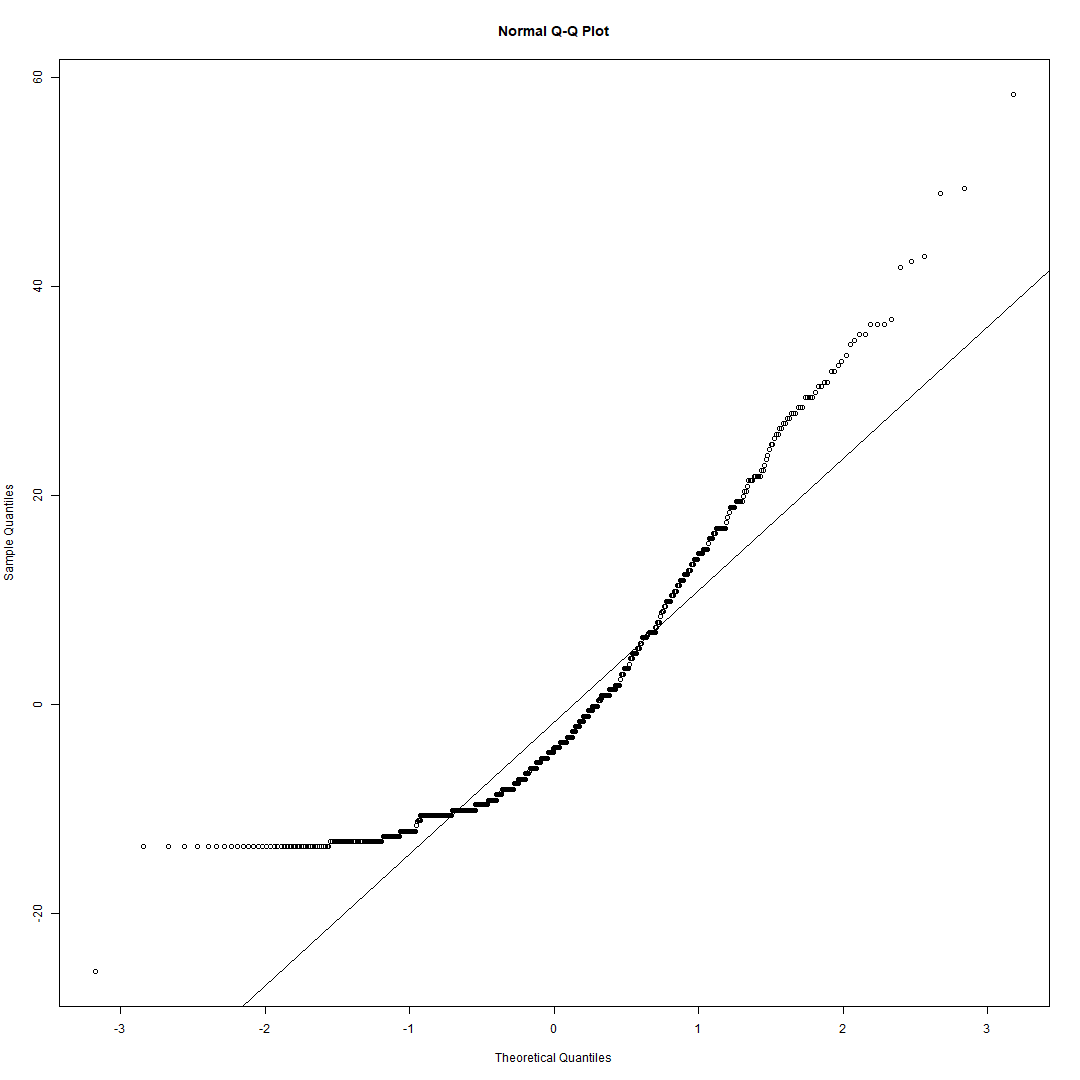
\includegraphics[width=300px, keepaspectratio]{resources/Anova1_Plot.png}
            \end{figure}
            \newpage
            \begin{figure}[h]
                \caption{QQPlot Μοντέλου ANOVA2 ($Yearsofresidence \sim PoliticalOrientation$)}
                \label{anova2plot}
                \centering
                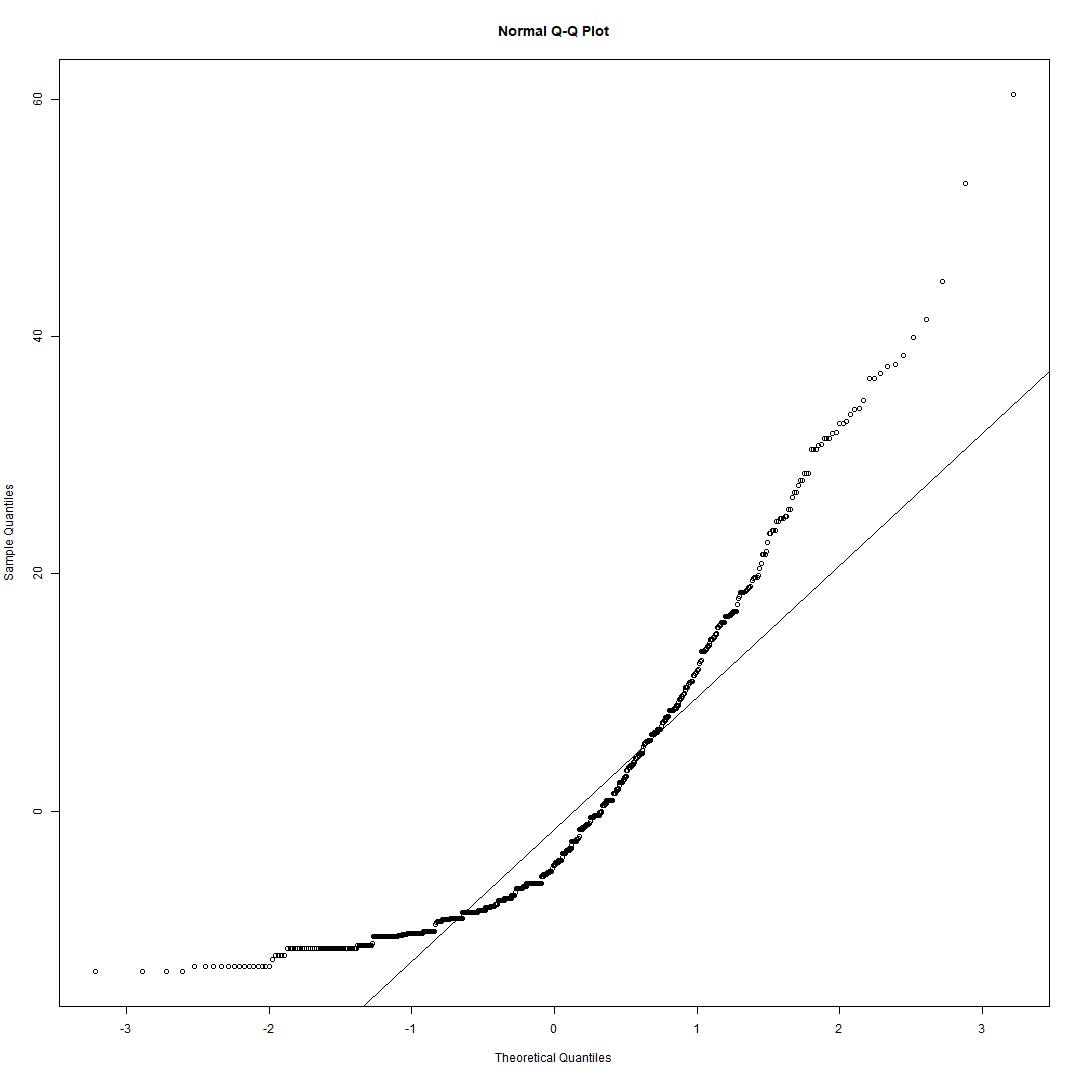
\includegraphics[width=300px, keepaspectratio]{resources/Anova2_Plot.png}
            \end{figure}
            \newpage
            \begin{figure}[h]
                \caption{QQPlot Πρώτου Μοντέλου Γραμμικής Παλλινδρόμησης}
                \label{model1plot}
                \centering
                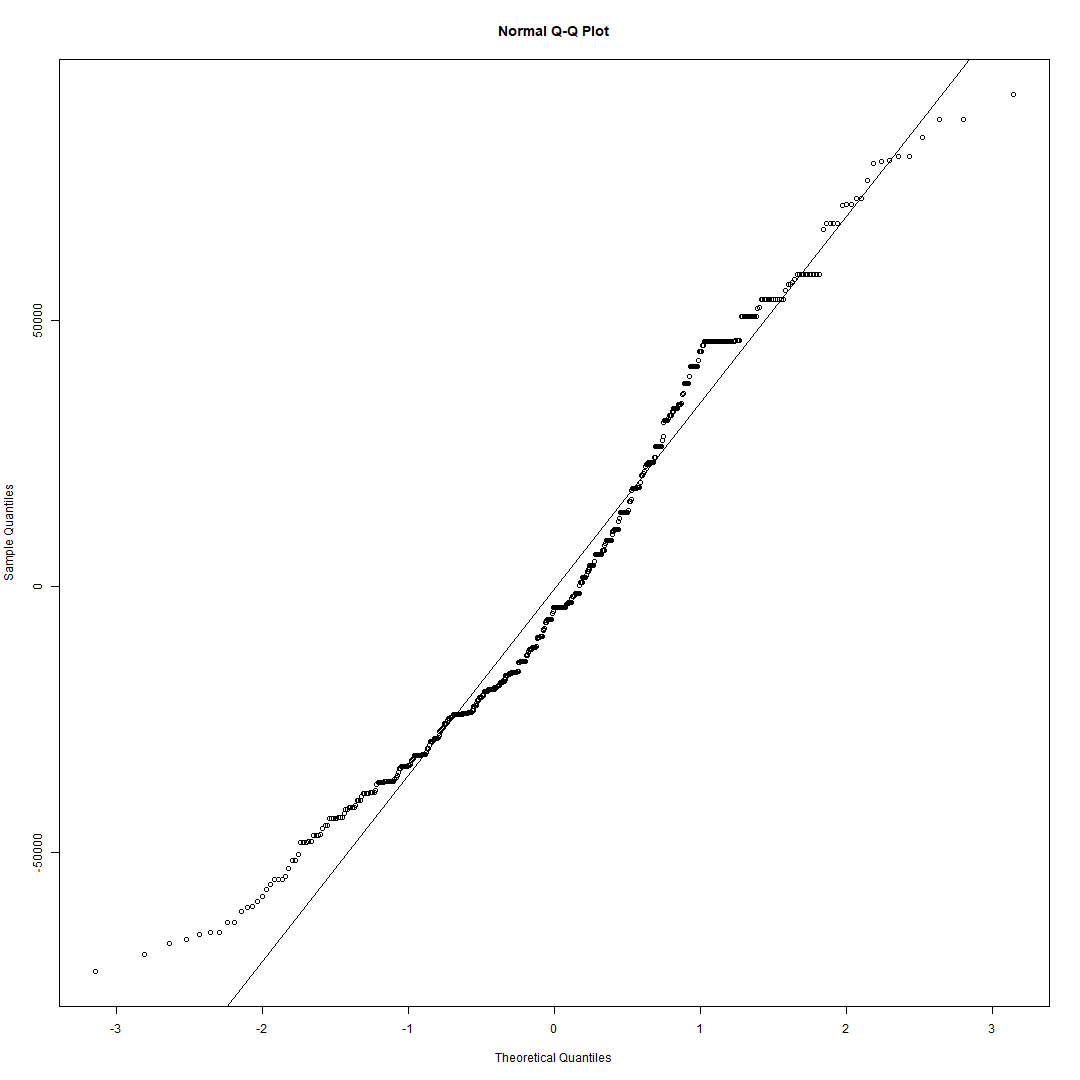
\includegraphics[width=300px, keepaspectratio]{resources/Model1_Plot.png}
            \end{figure}
            \newpage
            \begin{table}[h] 
                \setlength\extrarowheight{-3pt}
                \caption{Πίνακας Δευτέρου Μοντέλου Γραμμικής Παλλινδρόμισης} 
                \label{model2table}
                \begin{tabular}{@{\extracolsep{5pt}}lc} 
                    \\[-1ex]\hline 
                    \hline \\[-1ex] 
                     & \multicolumn{1}{c}{\textit{Dependent variable:}} \\ 
                    \cline{2-2} 
                    \\[-1ex] & Income \\ 
                    \hline \\[-1.8ex] 
                     Gender: female & $-$9,314.418$^{***}$ \\ 
                      & (2,380.520) \\ 
                      & \\ 
                     Marital\_Status: Widowed & $-$36,510.540$^{***}$ \\ 
                      & (4,692.898) \\ 
                      & \\ 
                     Marital\_Status: Divorced & $-$25,056.760$^{***}$ \\ 
                      & (3,611.607) \\ 
                      & \\ 
                     Marital\_Status: Separated & $-$30,188.590$^{***}$ \\ 
                      & (6,202.189) \\ 
                      & \\ 
                     Marital\_Status: Never married & $-$26,983.850$^{***}$ \\ 
                      & (2,918.340) \\ 
                      & \\ 
                     Marital\_Status: Partnered, not married \{VOL\} & 7,270.042 \\ 
                      & (9,038.889) \\ 
                      & \\ 
                     Constant & 73,793.870$^{***}$ \\ 
                      & (2,000.498) \\ 
                      & \\ 
                    \hline \\[-1ex] 
                    Observations & 874 \\ 
                    R$^{2}$ & 0.173 \\ 
                    Adjusted R$^{2}$ & 0.167 \\ 
                    Residual Std. Error & 34,363.650 (df = 867) \\ 
                    F Statistic & 30.149$^{***}$ (df = 6; 867) \\ 
                    \hline 
                    \hline \\[-1ex] 
                    \textit{Note:}  & \multicolumn{1}{r}{$^{*}$p$<$0.1; $^{**}$p$<$0.05; $^{***}$p$<$0.01} \\ 
                \end{tabular} 
            \end{table} 
            \newpage
            \begin{figure}[h]
                \caption{QQPlot Δευτέρου Μοντέλου Γραμμικής Παλλινδρόμησης}
                \label{model2plot}
                \centering
                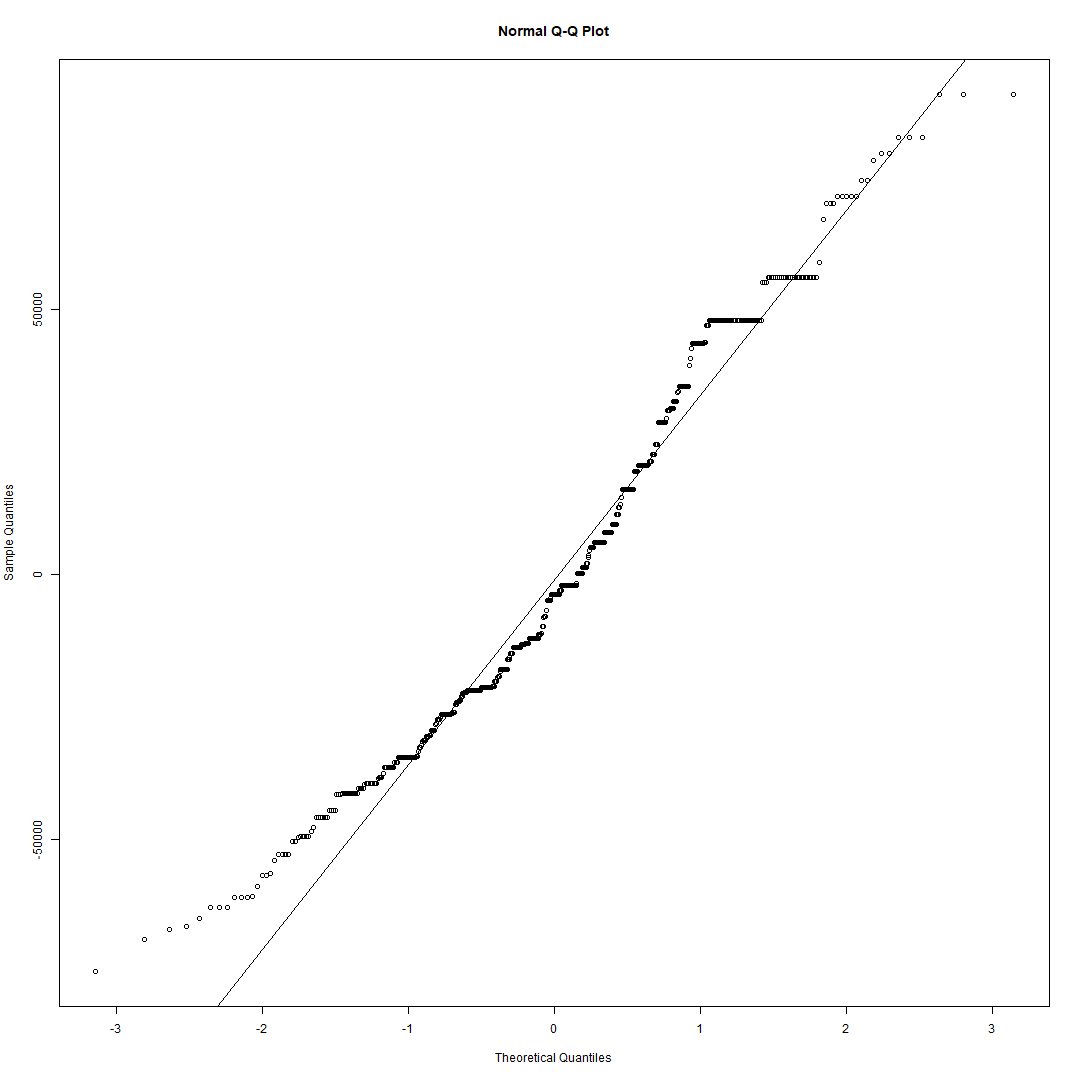
\includegraphics[width=300px, keepaspectratio]{resources/Model2_Plot.png}
            \end{figure}
            \end{center}
\bibliography{refs}{}
\bibliographystyle{plain}
\end{document}
